\documentclass[12pt]{article}
\usepackage[utf8]{inputenc}
\usepackage{graphicx}
\usepackage{lipsum}
\usepackage{amsmath}
\usepackage{amssymb}
\usepackage{amsthm}
\usepackage{enumitem}
\usepackage{tikz}
\usepackage{tikz-3dplot}
\usepackage{pgfplots}
\usepackage{graphicx}
\usepackage[a4paper, margin=1.91cm, top=1.91cm, bottom=1.91cm]{geometry}
\usepackage{hyperref}
\usepackage{glossaries}
\usepackage{tcolorbox}
\usepackage{mhchem}
\usepackage{cancel}
\usepackage{xcolor}
\usepackage{marginnote}
\usepackage{mathtools}
\usepackage{wrapfig}
\usetikzlibrary{calc}


\pgfplotsset{compat=newest}

\hypersetup{
    pdfauthor={Daniel Weronski Falcó},
    pdftitle={Environmental Physics PHYS50008},
    pdfsubject={Y2 Imperial College Environmental Physics Notes}
}
\title{Environmental Physics Notes}
\author{}
\date{}

\makeglossaries
\loadglsentries{glossary}

\begin{document}

\maketitle
\tableofcontents

\newpage
\section{Introduction}
\label{sec:introduction}

\subsection{Climate System Components}
There are 5 main components of the climate system:
\begin{itemize}
    \item \textbf{Atmosphere}: This has the fastest response time to changes in the climate system. 
    \item \textbf{Lithosphere}: This is comprised of the crust and the upper mantle (the top layers of the Earth). It 
    interacts mainly with the atmosphere through turbulent exchanges of mass e.g. desert dust storms, volcanic eruptions.
    \item \textbf{Hydrosphere}: This is comprised of all the water on Earth. It plays a key role on the climate by means
     of providing a heat reservoir due to its large mass and heat capacity. It also affects other components of the 
     climate system through the water cycle and affects other cycles such as the carbon cycle.
    \item \textbf{Cryosphere}: This is comprised of all the ice on Earth (ice sheets, glaciers, snow fields, sea ice). 
    It is important because it reflects a lot of solar radiation back into space. It also affects the 
    \hyperlink{glo:albedo}{albedo} of the Earth (by reducing it if its cryosphere's size decreases and vice versa).
    \item \textbf{Biosphere}: This is comprised of all the living organisms on Earth. It affects the climate system by 
    means of the carbon cycle and the water cycle. This is highly sensitive to climate state.
\end{itemize}

\begin{figure}[h]
    \centering
    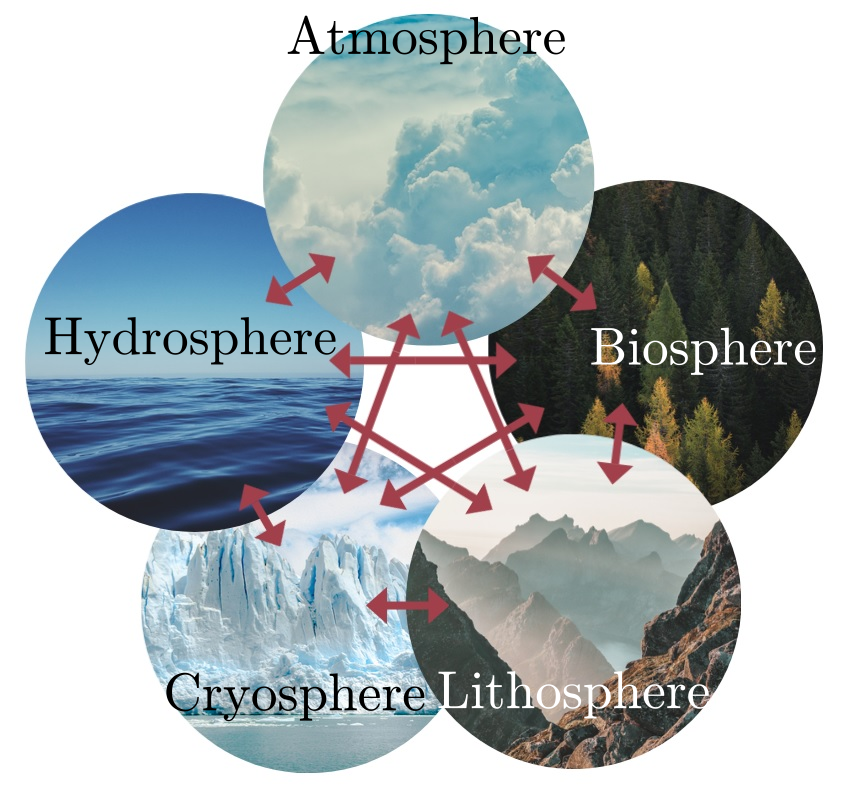
\includegraphics[scale=0.5]{figures/climate_system_components.png}
    \caption{Climate System Components}
    \label{fig:ClimateSystem}
\end{figure}

\subsection{Total Solar Irradiance}
The climate system is fundamentally driven by the sun. Energy transfer from the Sun to the Earth is only done through
EM radiation. To define this more rigorously, we assume the sun emmits \textbf{isotropically} (equally in all directions)
as a \textbf{black body}. We can reach an expression for the irradiance $I$ from the Sun reaching the \gls{TOA}:
$$
I = \sigma T_{\text{Sun}}^4 \frac{R_{\text{Sun}}^2}{R_{ES}^2} \quad \implies \quad \text{\hyperlink{glo:TSI}{TSI}} = \sigma 
T_{\text{Sun}}^4 \frac{R_{\text{Sun}}^2}{R_{ES}^2}
$$
where $\sigma$ is the Stefan-Boltzmann constant, $T_{\text{Sun}}$ is the temperature of the Sun, $R_{\text{Sun}}$ is the
radius of the Sun and $R_{ES}$ is the distance between the Earth and the Sun (radius of Earth's orbit, 1AU). A rough 
value for $I$ is $1360\ Wm^{-2}$.

Althought the \gls{TSI} is usually considered a constant, this does in fact vary on a number of timescales.
There are millenial time-scale orbital variations (Milankovitch cycles) and the Sun's own activity cycle (11 years). 
The \gls{TSI} can be measured in a number of ways, most recently by satellite measurements. The variation in 
the \gls{TSI} seen over the last few decades is of the order 1-2 $Wm^{-2}$.

\subsection{Planetary Albedo and the Earth's Emitting Temperature}
\label{sec:albedo}
At the \gls{TOA}, the only energy transfer is through EM (photon) radiation. Over time, the Earth will reach
\textbf{radiative equilibrium} where the amount of energy absorbed by the Earth is equal to the amount of energy emitted
by it at the \gls{TOA}.

\noindent Not all the energy from the Sun is absorbed by the Earth. Some of it is reflected back into space. The fraction
of energy reflected back into space is called the {\textbf{\hyperlink{glo:albedo}{planetary albedo}}}. 

The Earth, with radius $R_E$ and area $\pi R_E^2$ incident to the solar beam with \hyperlink{glo:albedo}{albedo} $\alpha_p$ 
will reach equillibrium when:
$$
4 \pi R_E^2 \sigma T_E^4 = (1 - \alpha_p) \pi R_E^2 \text{\hyperlink{glo:TSI}{TSI}} \quad \implies \quad T_E = \left(
\frac{1 - \alpha_p}{4} \right)^{\frac{1}{4}} T_{\text{Sun}} \approx 255\ K
$$

Here, we have equated the Earth's emission to the energy absorbed by it. Rearanging, we obtain the \textbf{emitting
temperature} ($T_E$) of the Earth which comes out to about $\sim 255$ K. This is much lower than the actual average surface
temperature of the Earth ($\sim 288$ K). We will see later in the course that this is because the Earth in fact has an 
atmosphere which traps heat and increases the surface temperature as to balance the energy equation.

\newpage
\section{The Greenhouse Effect}
\label{greenhouse_effect}

Up to now we have considered a very crude model in which the Earth is a black body with no atmosphere, and its energy 
balance is ruled by the incoming solar radiation and the outgoing long wave radiation (\gls{LW}). We have seen
that such a model gave us a temperature that is significantly below the one that we observe. This is due to the 
\textbf{greenhouse effect}.

\subsection{Emissivity, Absorptivity and Transmissivity}
We can now come up with a more nuanced model of the Earth's energy balance. First we need to consider that materials are
not perfect emitters, so we definte the \textbf{\gls{emissivity}} $\epsilon_\lambda$ of 
a material as the ratio of the irradinace emitted by the material to the irradiance emitted by a black body at the same
temperature. Notice that the \gls{emissivity} is a function of wavelength. 
$$
\epsilon_\lambda = \frac{I_{\text{material}}}{I_{\text{black body}}}
$$

By definition, a black body has an \gls{emissivity} of $\epsilon_{BB} = 1$ so it follows that 
$I_{\text{material}} = \epsilon_\lambda \sigma T^4$. A material that emits like a \textbf{grey body} is one that has a 
constant \gls{emissivity} across all wavelengths. \\

\noindent We can also define the \textbf{\gls{absorptivity}} $a_\lambda$ of a
material as the ratio of the irradiance actually absorbed by the material to the irradiance incident on it. This is also
a function of wavelength and is always a number between 0 and 1, meaning actual materials absorb less than a black body.
It follows that, by definition, the \gls{absorptivity} of a black body is 
$a_{BB} = 1 = \epsilon_\lambda$ and in general (for systems in local thermodynamical equillibrium, as per Kirchoff's Law)
$a_\lambda = \epsilon_\lambda$.\\

\noindent Finally, the more absorbing a material is, the less radiation it will transmit. We define the 
\textbf{\gls{transmissivity}} $t_\lambda$ of a material as $1 - a_\lambda = 1 - \epsilon_\lambda$.
 This is also a function of wavelength and is always a number between 0 and 1. This relationship only
holds in the absence of scattering, a reasonable assumption for clear-sky \gls{LW} radiation.

\subsection{Optical Depth}
\label{sec:opticaldepth}

We can also write transmissivity in terms of the \hyperlink{glo:opticaldepth}{optical depth} $\tau_\lambda$ of a
material as follows:
$$
t_\lambda = e^{-\tau_\lambda} \quad \implies \quad \tau_\lambda = \int_0^\infty k_{a \lambda} \rho_{a} dz
$$
where \hypertarget{absorption_coefficient}{$k_{a \lambda}$} is the \textbf{absorption coefficient} of the material, 
$\rho_a$ is the density of the material across the atmosphere $dz$. 

The optical depth is dimensionless: it the atmosphere
has a $\tau$ of 1 it means that the amount of radiation transmitted through it from the surface to the \gls{TOA}
is reduced by a factor of $1/e$. Increasing the amount of absorbing material in the atmosphere will increase $\tau_\lambda$
and therefore reduce $t_\lambda$.

\subsection{Deffinition of, and a Simple Model of the Greenhouse Effect}
\label{sec:greenhouse_definition}
We will define the \textbf{greenhouse effect} ($G$) as the amount of \gls{LW} radiation emitted by the Earth's
surface that is trapped within the Earth's atmosphere. We can see how the atmosphere interacts with \gls{LW}
and \gls{SW} radiation in figure \ref{fig:transmitted_radiation}.

\begin{figure}[h]
    \centering
    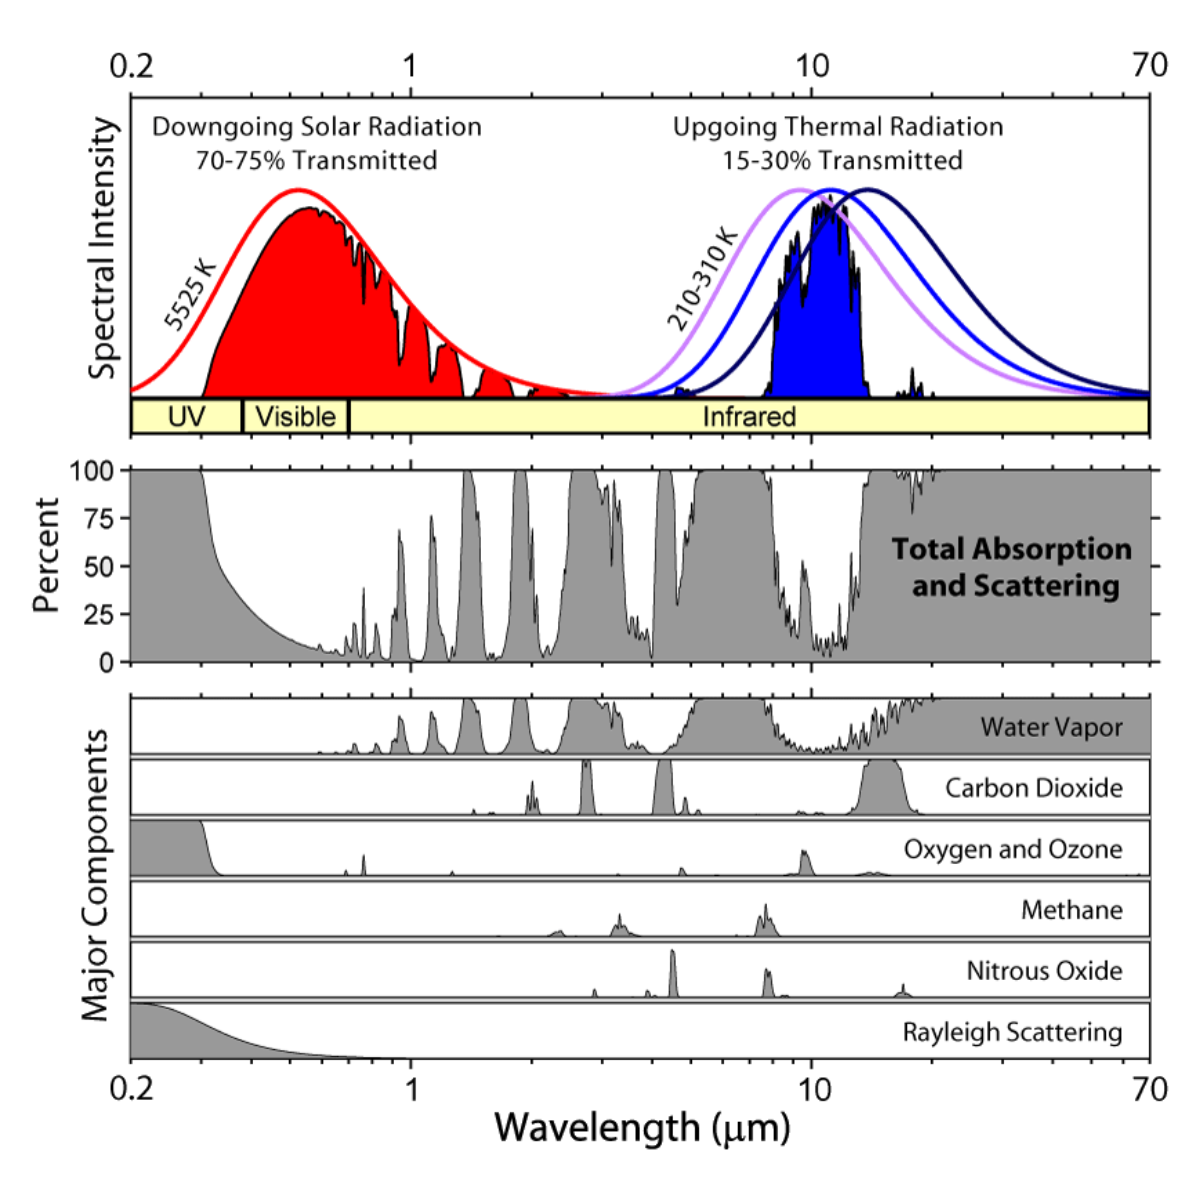
\includegraphics[width=0.65\textwidth]{figures/transmitted_radiation.png}
    \caption{Radiation Transmitted by the Atmosphere.}
    \label{fig:transmitted_radiation}
\end{figure}

As per figure \ref{fig:transmitted_radiation}, the atmosphere is much more transparent to \gls{SW} radiation than
it is to \gls{LW} radiation. Water vapour is the main absorber of \gls{LW} radiation followed by
carbon dioxide and some other gases. If we assume the Earth's surface has a temperature $T_s$ and it emmits as a black
body, then we can define $G$ as:
$$
\boxed{
    G = \sigma T_s^4 - \text{\gls{OLR}}
}
$$
where \gls{OLR} is the \textbf{outgoing long wave radiation} at the \gls{TOA}, i.e. the sum total
of radiation that escapes Earth into space.\\

\noindent Let us introduce a simple model of the greenhouse effect. We will have a few (important) assumptions:
\begin{itemize}
    \item The atmosphere is completely transparent to \textbf{solar radiation} (\gls{SW}).
    \item We have blackbody emissioin from the surface at temperature $T_s$.
    \item The atmosphere is a single layer grey-body with \gls{emissivity} $\epsilon_a$ and
    temperature $T_a$ emitting in the upward and downward directions equally.
    \item There is \textbf{radiative equillibrium} at the surface, in the atmosphere and at the \gls{TOA}.
\end{itemize}

In this case, by energy conservation we can write the following for the \textbf{top of the atmosphere}:
\begin{equation}
    \begin{aligned}
    &\begin{tabular}{c}
    Incoming \\ \gls{SW} from the Sun
    \end{tabular}
    & = 
    &\begin{tabular}{c}
    \gls{LW} emitted \\ by the atmosphere
    \end{tabular}
    & + 
    &\begin{tabular}{c}
    Transmitted \\ \gls{LW} from the surface
    \end{tabular} \\
    &\makebox[3.7cm]{$\displaystyle\frac{(1 - \alpha_p)\ \text{\gls{TSI}}}{4}$} & = &\makebox[4cm]{$\epsilon_a 
    \sigma T_a^4$} & + &\makebox[4cm]{$(1 - \epsilon_a) \sigma T_s^4$}
    \end{aligned}
    \nonumber
\end{equation}
\textbf{within the atmosphere} we can write:
\begin{equation}
    \begin{aligned}
    &\begin{tabular}{c}
    \gls{LW} emitted by the \\ surface absorbed by atmos
    \end{tabular}
    & = 
    &\begin{tabular}{c}
    \gls{LW} emitted by the \\ atmosphere up and down
    \end{tabular}\\
    &\makebox[5.5cm]{$\displaystyle\epsilon_a \sigma T_s^4$} & = &\makebox[5cm]{$2 \epsilon_a \sigma T_a^4$}
    \end{aligned}
    \nonumber
\end{equation}
finally, \textbf{at the surface} we can write:
\begin{equation}
    \begin{aligned}
    &\begin{tabular}{c}
    \gls{LW} emitted \\ by the surface    
    \end{tabular}
    & = 
    &\begin{tabular}{c}
    Incoming \\ \gls{SW} from the Sun
    \end{tabular}
    & + 
    &\begin{tabular}{c}
    \gls{LW} emitted by the \\ atmosphere downwards
    \end{tabular} \\
    &\makebox[3cm]{$\displaystyle\sigma T_s^4$} & = &\makebox[4cm]{$\displaystyle\frac{(1 - \alpha_p)\ 
    \text{\gls{TSI}}}{4}$}& + &\makebox[4.5cm]{$\epsilon_a \sigma T_a^4$}
    \end{aligned}
    \nonumber
\end{equation}

\noindent With these we have a set of simultaneous equations with which we can solve for $T_s$ and $T_a$ for some given
reasonable values for $\alpha_p$, $\epsilon_a$ and \gls{TSI}. We can solve for $T_s$ and $G$ as follows:
\begin{equation}
    \begin{aligned}
    T_s &= \left(\frac{(1 - \alpha_p)\ \text{\gls{TSI}}}{2 \sigma (2 - \epsilon_a)}\right)^{1/4} \\
    \text{\gls{OLR}} &=  \epsilon_a \sigma T_a^4 + (1 - \epsilon_a)\sigma T_s^4 \\
    G &= \sigma T_s^4 - \text{\gls{OLR}}\\
    &= \epsilon_a \sigma T_s^4 - \epsilon_a \sigma T_a^4
    \end{aligned}
    \nonumber
\end{equation}
having used the definition of $G = \sigma T_s^4 - \text{\gls{OLR}}$ and the first equation above for the 
\gls{TOA} balance being in equillibrium (i.e. $\text{\gls{OLR}} = $ incoming \gls{SW} from the
Sun).

With a further substitution from the atmospheric balance (2nd equation above) for $T_a$ we can write:
$$
\boxed{
G = \frac{\epsilon_a}{2} \sigma T_s^4
}
$$
which is what we expect: a thicker, more absorbing atmosphere will have a lower \gls{transmissivity}
meaning a higher \gls{emissivity} ($\epsilon_a$) meaning a stronger greenhouse effect $G$.

\newpage
\section{Radiative Forcing and Feedback}
\label{sec:forcing_feedback}
\subsection{Radiative Forcings and Feedbacks}
Let $I_N$ be the net irradiance at the \gls{TOA}, defined positive in the downward direction. It
follows that in \textbf{radiative equillibrium}:
$$
I_N = \frac{(1 - \alpha_p) \text{\gls{TSI}}}{4} - \text{\gls{OLR}} = 0
$$

\begin{itemize}
    \item A \textbf{radiative forcing} ($\Delta Q_{EXT}$) is an external perturbation to the climate system away from 
radiative equillibrium at the \gls{TOA}. A positive forcing leads to a positive global mean surface temperature
change ($\Delta T_s$), and vice versa.
    \item A \textbf{feedback} ($\Delta Q_{INT}$) is an internal process which responds to the forcing \textbf{and} has an
    effect on the global mean surface temperature.
\end{itemize}

\noindent It follows from the above definitions that:
\begin{align}
    \text{In the \textbf{absence} of feedback processes} \quad \Delta I_N &= \Delta Q_{EXT} \nonumber \\
    \text{In the \textbf{presence} of feedback processes} \quad \Delta I_N &= \Delta Q_{EXT} + \Delta Q_{INT} \nonumber
\end{align}

We can also define a further parameter, the \textbf{climate feedback parameter} $\lambda$. This is a measure 
of how much the planet's energy balance responds to changes in global mean surface temperature $\Delta T_s$. It is a
measure of how much additional energy is trapped or lost as a result to said change in surface temperature. We define
the total \textbf{climate feedback parameter} $\gamma$ as:
$$
\Delta Q_{INT} = \gamma \Delta T_s \label{eq:gamma}
$$
where $\gamma$ represents the radiative response of the climate feedback to a given $\Delta T_s$. Its units are 
$\text{W m}^{-2} \text{K}^{-1}$.

\subsection{Decomposing the Feedback Parameter}
\label{sec:decompose_feedback}
We can decompose the total feedback parameter $\gamma$ into the sum of individual feedback parameters:
$$
\gamma = \frac{dI_N}{dT_s} = \frac{\partial I_N}{\partial T_s} + \sum_x \frac{\partial I_N}{\partial x} 
\frac{\partial x}{\partial T_s}
$$
where $x$ represents the various parameters (e.g. water vapour). Here, $\frac{\partial I_N}{\partial T_s} = -\gamma_{BB}$
is the \textbf{blackbody feedback parameter}. The negative sign is simply to represent the fact that the surface will 
radiate more more energy as it warms, reducing the net irradiance at the \gls{TOA} ($I_N$).

\begin{tcolorbox}
    \textbf{Example:\\}
    For a simple 1 layer atmosphere transparent to solar radiation, it follows that $\text{\gls{OLR}} = \epsilon ' \sigma T_s^4$
    where $\epsilon '$ is the effective \hyperlink{glo:emissivity}{emissivity} which reduces with atmospheric 
    \hyperlink{glo:absorptivity}{absorptivity} and hence \hyperlink{glo:emissivity}{emissivity} increases. We can write:
    $$
    \frac{\partial I_N}{\partial T_S} = -\frac{\partial\ \text{\gls{OLR}}}{\partial T_s} = -\gamma_{BB} \quad \implies \quad
    \boxed{\gamma_{BB} = 4 \epsilon ' \sigma T_s^3}
    $$
\end{tcolorbox}

As per the example above, it becomes apparent that for a parameter ($x$) to exert a strong feedback, it must be dependent
on both $T_s$ \textbf{and have an influence on} the net irradiance at the \gls{TOA} ($I_N$). 

\subsection{Water Vapour Feedback and Clausius-Clapeyron Scaling}
\label{sec:clausius-clapeyron}

We mention in section \ref{sec:greenhouse_definition} that water vapour is the main absorber or \gls{LW} radiation, and 
therefore the most important greenhouse gas. Water vapour concentrations show a strong dependence on temperature, i.e.
the warmer the atmosphere, the more water vapour it can hold. This is a result of the Clausius-Clapeyron relation.\\

As per Paterson's thermodynamics course, we know that the pressure of water vapour which is saturated with respect to 
liquid water at a given temperature $T$ is given by:
$$
\frac{dP_s}{dT} = \frac{s_v - s_l}{v_v - v_l} \quad \implies \quad \boxed{\frac{dP_s}{dT} = \frac{l_v}{T v_v}}
$$
at the vapour-liquid phase boudary where $s_v$ and $s_l$ are the specific entropies of vapour and liquid water respectively,
$v_v$ and $v_l$ are the specific volumes of vapour and liquid water respectively, $l_v$ is the latent heat of
vaporisation and $P_s$ is the saturation vapour pressure.

If we assume water vapour behaves as an ideal gas, it is apparent that $P_s v_v = Nk_B T/Nm_v = k_B T / m_v$ where $m_v$ is
the molecular mass of water (remember we are using specific volume, not volume). We can define the gas constant for water
vapour $R_v = R_v = k_B / m_v$ and hence:
$$
\frac{dP_s}{dT} = \frac{P_s l_v}{R_v T^2} \quad \implies \quad \frac{dP_s}{P} = \frac{l_v}{R_v T^2}dT
$$
for context, we find that for sensible values for the constants:
$$
\frac{\left(\frac{dP_s}{P_s}\right)}{dT_s} \approx 0.07\ \text{K}^{-1}
$$
we call this the Clausius-Clapeyron scaling. Note that this does not apply to the actual vapour pressure (related to
the absolute amount of water vapour in the atmosphere). Vapour pressure and saturation vapour pressure are related by:
$$
\text{Relative Humidity, RH} = \frac{P_v}{P_s} \times 100\% \quad \implies \quad +7\%\ \text{RH per degree warming}
$$
where $P_v$ is the vapour pressure. 

Climate models suggest that relative humidity is conserved under anthropogenic climate change meaning that the absolute 
amount of water vapour in the atmosphere increases as atmospheric temperature increases.


\newpage
\section{Water in the Climate System}
\label{sec:water_in_climate}

Figure \ref{fig:soden_held} shows us the radiative feedback of various parameters (see section \ref{sec:forcing_feedback}).
In this section we will focus on how these parameters lead to a positive or negative radiative feedback.

\begin{figure}[h]
    \centering
    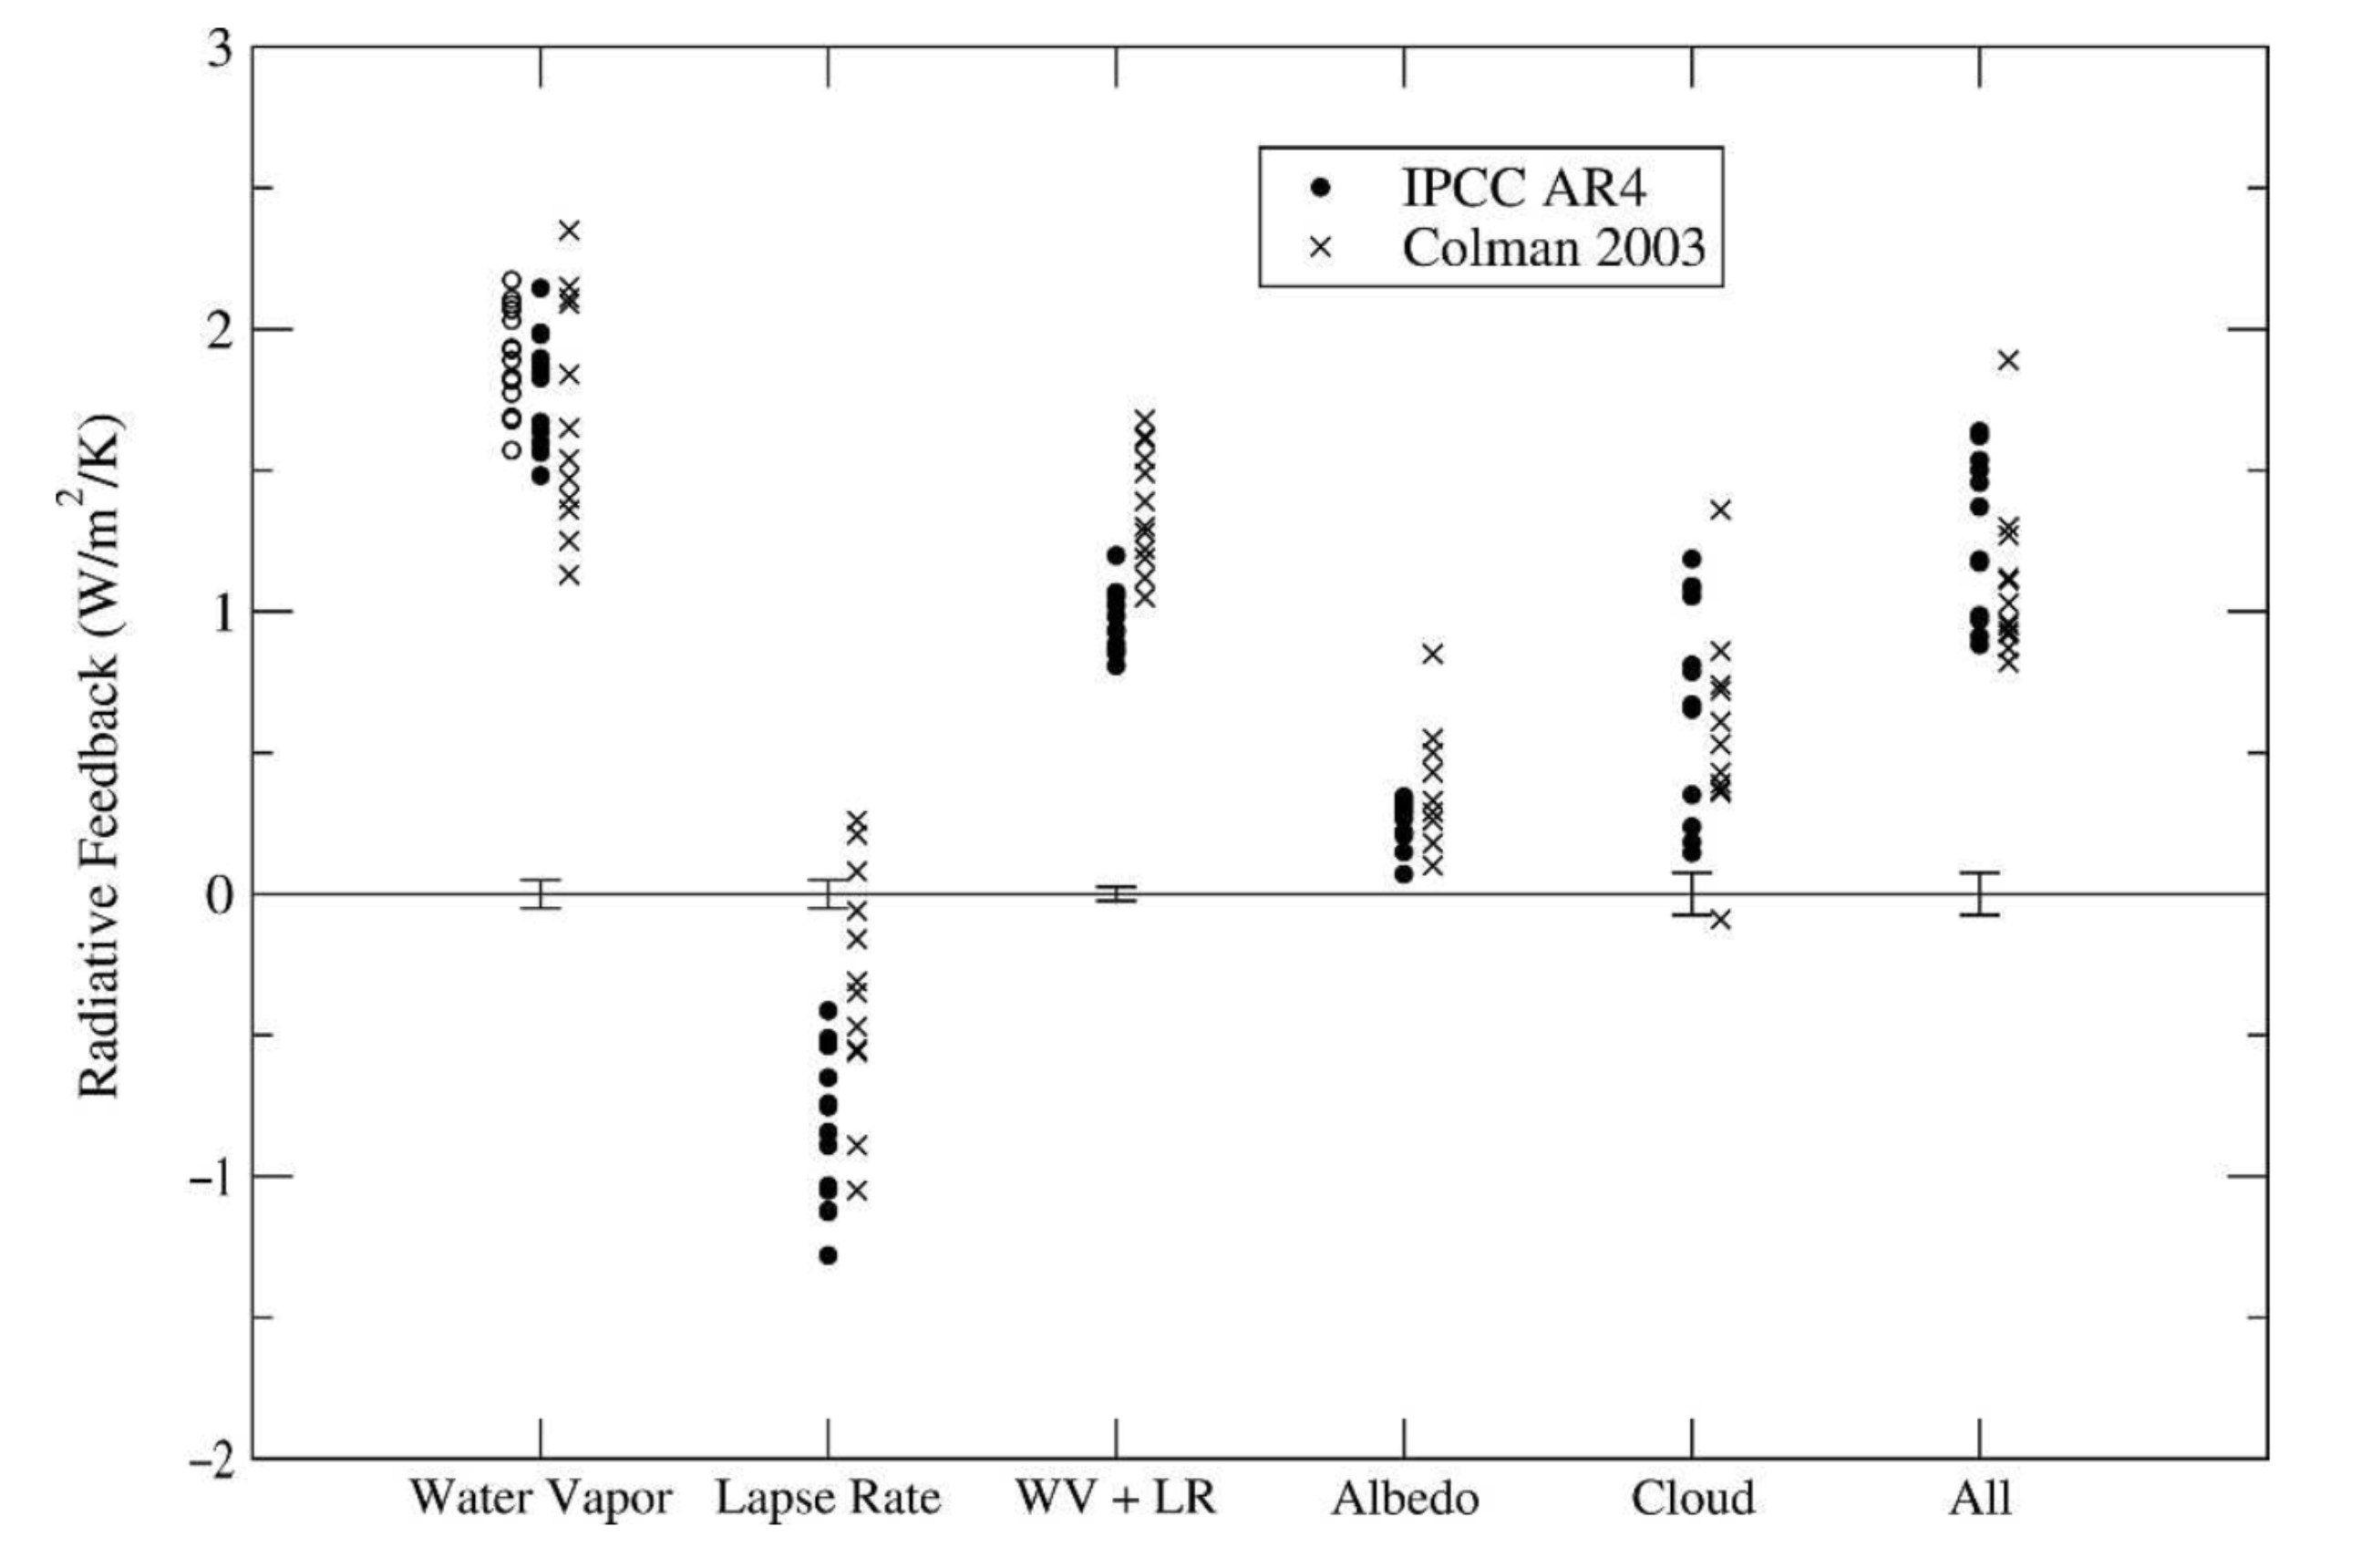
\includegraphics[width=0.75\textwidth]{figures/Soden and Held 2006.png}
    \caption{Radiative Feedback of Various Parameters (\cite[Soden and Held 2006]{soden_held_2006}).}
    \label{fig:soden_held}
\end{figure}

\subsection{Ice-Albedo Feedback}
\label{sec:ice_albedo_feedback}

The distribution of sea-ice shows a natural seasonability linked to the pattern of solar radiation at the surface with a
maximum etent at both poles after their respecive polar nights (and vice versa). Over the last few decades, satellite
observations have shown a clear decrease in the extent of sea-ice in the arctic (this is not the case in the Antarctic,
where the pattern seen is different. There is no clear sign of decreasing of sea-ice, in fact there are signs of a slight
increase. The reasons why are still up for debate and more recent data post 2017 show a decrease as expected with the
warming of the climate. This is non-examinable).

The \textbf{ice-albedo feedback} mechanism suggests that an increase in surface temperature would result in a reduced 
snow and sea-ice cover and hence reduce \hyperlink{albedo}{surface albedo} ($\alpha$). This would result in a decrease in
planetery albedo $\alpha_p$ and hence an increase in absorbed solar radiation. This would lead to a further increase in
surface temperature and so on. This is a \textbf{positive feedback} mechanism as shown in Figure \ref{fig:soden_held}.

\subsection{Lapse Rate}
\label{sec:lapse_rate}

The \textbf{lapse rate} is the negative rate at which temperature changes with height in the atmosphere. In the troposphere,
where the temperature decreases with height, the lapse rate is positive. We define lapse rate $\Gamma$ as:
$$
\Gamma = -\frac{dT}{dz}
$$
where $T$ is temperature and $z$ is height.

For a parcel of dry air lifted in an atmosphere due to convection, it follows that it does so adiabatically. In this case
we say that it rises at the \textbf{dry adiabatic lapse rate} $\Gamma_d$. 
$$
c_PdT - vdP = dq \quad \text{1st Law of Thermodynamics} \\
$$
$$
\frac{dT}{dz} = - \frac{g}{c_P} \quad \implies \quad \boxed{\Gamma_d = \frac{g}{c_P}}
$$

The same thing happens for a parcel of moist air. We begin by imagining a parcel 
of air near the surface that contains some non-zero amount of water vapour. As the
parcel rises, it cools adiabatically so it gets closer and closer to its saturation
point. Eventually it does, and the height at which it reaches the saturation point
is called the \textbf{lifting condensation level (LCL)}. At this point, the parcel
condenses and releases latent heat as it rises further. This heat means the parcel's
temperature does not decrease as fast as it otherwise would. Such a parcel is said
to be following the \textbf{moist adiabatic lapse rate} $\Gamma_s$.

% Make z-T diagram showing dry and moist adiabatic lapse rates showing the difference in slopes and the LCL
\begin{figure}
    \centering
    \begin{tikzpicture}
        \begin{axis}[
            xlabel=$T$,
            ylabel=$z$,
            xmin=0, xmax=10,
            ymin=0, ymax=10,
            % xtick={},
            % ytick={},
            yticklabels={},
            xticklabels={},
            axis lines=middle,
            axis line style={-},
            width=0.7\textwidth,
            height=0.7\textwidth,
            grid=major,
            grid style={dashed, gray!30},
            % legend pos=north east,
            % legend style={font=\small, cells={align=left}},
            % legend cell align={left},
        ]
        \addplot[domain=1:5, samples=100, color=blue]{-1.5*x + 10}
        node[pos=0, above]{$\Gamma_s$};

        \addplot[domain=1:9, samples=100, color=red]{-0.5*x + 5}
        node[pos=0, above]{$\Gamma_d$};

        \addplot[dotted, thick, domain=2:8, samples=100, color=black]{2.5}
        node[pos=0.5, above right]{$LCL$};
        \end{axis}
    \end{tikzpicture}
    \caption{Dry and Moist Adiabatic Lapse Rates.}
    \label{fig:adiabatic_lapse_rates}
\end{figure}

We can combine the two lapse rates into one equation as follows (see handout 2, moist adiabatic lapse rate for derivation):
$$
\Gamma_s = \Gamma_d \frac{1 + \frac{w_s l_v}{R_d T}}{1 + \frac{\epsilon l_v^2 w_s}{c_p R_d T^2}} = \Gamma_d \frac{1+X}{1+bX}
$$
where $l_v$ is the latent heat of vapourisation, $w_s$ is the \textbf{saturation mixing ration}, $T$ is the temperature,
$R_d$ is the gas constant for dry air, $c_p$ is the specific heat capacity of dry air at constant pressure, $\epsilon$ is
the ratio of the gas constants for dry air and water vapour, $X = \frac{w_sl_v}{R_dT}$ and $b = \frac{\epsilon l_v}{c_pT}$.

To summarise, and worth noting is the following:
$$
\boxed{\Gamma_d = \frac{g}{c_p}\ , \quad b > 1 \ , \quad \Gamma_s < \Gamma_d}
$$

\subsection{Lapse Rate Feedback}
\label{sec:lapse_rate_feedback}

We showed in section \ref{sec:lapse_rate} that the rate of change of $\Gamma_s$ with temperature must be negative. In 
regions of high moisture and convective uplift (e.g. tropical troposphere) a change in surface temperature will in turn
lead to a change in the atmosperic temperature at higher altitudes. If we have a radiative \hyperlink{glo:forcing}{forcing}
which results in a surface warming, this will lead to a decrease in $\Gamma_s$ (the gaph in Figure \ref{fig:lapse_rate_feedback}
gets steeper). In other words the temperature at higher altitudes will increase more than ``expected'', the graph does
not simply translate. We can see this in Figure \ref{fig:lapse_rate_feedback}.

\begin{figure}
    \centering
    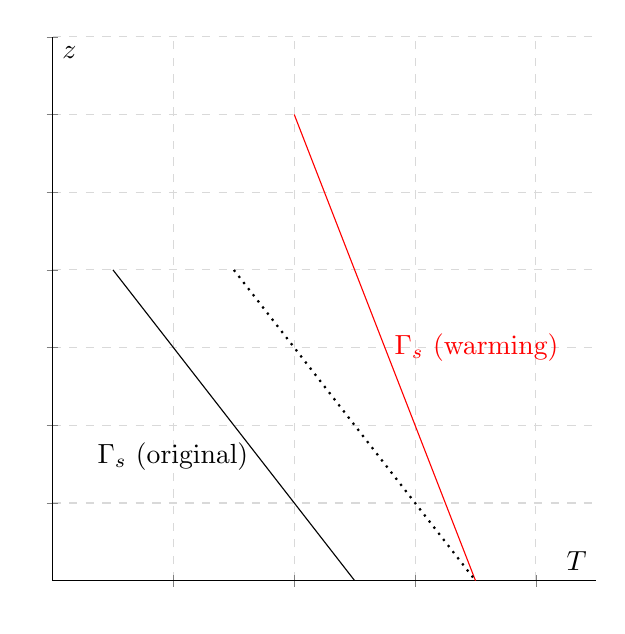
\begin{tikzpicture}
        \begin{axis}[
            xlabel=$T$,
            ylabel=$z$,
            xmin=0, xmax=9,
            ymin=0, ymax=7,
            % xtick={},
            % ytick={},
            yticklabels={},
            xticklabels={},
            axis lines=middle,
            axis line style={-},
            width=0.7\textwidth,
            height=0.7\textwidth,
            grid=major,
            grid style={dashed, gray!30},
            % legend pos=north east,
            % legend style={font=\small, cells={align=left}},
            % legend cell align={left},
        ]
        \addplot[domain=4:7, samples=100, color=red]{-2*(x - 2) + 10}
        node[pos=0.5, right]{$\Gamma_s$ (warming)};

        \addplot[domain=1:9, samples=100, color=black]{-x + 5}
        node[pos=0.3, left]{$\Gamma_s$ (original)};

        \addplot[dotted, thick, domain=3:7, samples=100, color=black]{-x + 7};
        % node[pos=0, above]{$\Gamma_s$};

        \end{axis}
    \end{tikzpicture}
    \caption{Lapse Rate Feedback.}
    \label{fig:lapse_rate_feedback}
\end{figure}

Figure \ref{fig:lapse_rate_feedback} shows that the lapse rate feedback is negative. This means that a radiative forcing
will lead to a greater change in temperature at higher altitudes than expected. This is a positive feedback because
the change in temperature at higher altitudes will lead to a greater \gls{LW} emission at the \gls{TOA} (equivalently,
an increase in \gls{OLR}) and also a net decrease in \gls{LW} emission back towards the surface. This will therefore 
lead to a cooling of the surface, hence negative feedback.

\subsection{Lapse Rate and Water Vapour Feedback Combined}
\label{sec:lapse_rate_water_vapour_feedback}

We have seen in section \ref{sec:clausius-clapeyron} that relative humitidy tends to be conserved i.e. if atmospheric
temperature increases or decreases, the relative humidity stays the same meaning the absolute levels of water in the air
increase or decrease respectively. This is a consequence of Clausius-Clapeyron scaling (again, see section 
\ref{sec:clausius-clapeyron} for the details).

A higher absolute level of water vapour in the air also means a higher latent heating once saturation point is reached 
(there is more water per unit volume that condenses, so more heat released per unit volume). This means that the 
water vapour and lapse rate are intimately related. More water vapour means a lower lapse rate due to increase in 
temperature, and a lower lapse rate means more heat is radiated out to space. Overall the combined feedback is positive,
see figure \ref{fig:soden_held}.

\subsection{The Impact of Clouds on Radiation}
\label{sec:clouds_radiation}

Clouds interact strongly with both \gls{SW} and \gls{LW} radiation. They are highly reflective to \gls{SW} radiation
(they are responsible for ~50\% of the Earth's \gls{albedo}) and are also strong absorbers and emitters of \gls{LW}. 
However the net impact is highly dependent on a few factors.\\

In the presence of sunlight, clouds have a very reflective effect on \gls{SW} radiation compared to clear-sky conditions,
especially if they are over a dark surface (e.g. ocean or vegetation). 

If the cloud is at a low altitude, this cloud is hot and therefore a good blackbody emitter so there is a net loss of 
energy to space. The cloud therefore cools the surface.

If the cloud is at a high altitude, this cloud is cold and therefore does not emit much \gls{LW} radiation. The \gls{LW}
effect will dominate over the \gls{SW} effect and the cloud will act as a blanket, trapping heat and warming the surface.

At night, all clouds (due to their relatively high optical thickness) they always act as a blanket, trapping heat and
warming the surface (or rather not letting it cool as much as it otherwise would).\\

% Place the following in a box
\begin{tcolorbox}
\noindent In general we will think of a low cloud = cooling, high cloud = warming with the exception of night time we
noted before.
\end{tcolorbox}

Note that the above is a very simplified picture. In reality, clouds are highly variable in their optical thickness (our
main assumption was that clouds are very thick) and they have all sorts of microphysical properties which affect their
feedback properties. The value of the cloud feedback parameter $\gamma_c$ is the most uncertain one and varies significantly
between models.\\

\noindent From our simple model we can write the following equation for the cloud feedback parameter:
$$
\boxed{\gamma_c = \frac{\partial I_N}{\partial x}\frac{\partial x}{\partial T_s}}
$$
where the first term depends on cloud altitude, time of day/year, cloud microphysics and otherwise. The second term is
a non-trivial relationship between cloud properties and temperature.


\newpage
\section{The Carbon Cycle}
\label{sec:carbon-cycle}

\newcommand{\COtwo}{CO\textsubscript{2}\ }  % Carbon Dioxide

\subsection{Fast and Slow Carbon Cycle}
\label{sec:fast-slow-carbon}

\begin{itemize}
    \item \textbf{Fast Carbon Cycle:} This is the flow of carbon from a reservoir or store to another where each cycle 
    takes about 10s of years. This tends to include the atmopshere, biosphere, soils and upper ocean. These stores are
    relatively small. 

    Anthropogenic changes in the stores are relatively small when compared to natural cycles, but still disturb the 
    natural balance of the cycle

    \item \textbf{Slow Carbon Cycle:} This is the flow of carbon from a reservoir or store to another where each cycle
    takes 100,000s of years. This tends to include the deep ocean and geological sediments (e.g. fossil fuel reseroirs
    or carbonate rocks like limestone). These stores are relatively large.
\end{itemize}

\subsection{Atmospheric Carbon Dioxide Concentrations, Emissions and Uptake}
\COtwo concentration is something that has changed over time due to natural and anthropogenic factors. Concentrations
are higher today than they have been at any point in the last 400,000 years. Over the last 1000 years up until 1750 (the
start of the industrial revolution) \COtwo concentrations were relatively stable at $\sim$285ppm. Since then they have
increased to the current level of $\sim$415ppm. 

Over this period, \COtwo has been the largest contributor to the total anthropogenic radiative forcing. This is a result
of the increase in \COtwo concentration in the atmosphere, its strong absorption peak at 15\textmu m and its long 
atmospheric lifetime.\\

Anthropogenic emissions of \COtwo are mainly due to the burning of fossil fuels and cement production. We can combine 
the net increase in \COtwo concentration in the atmosphere by considering the emissions and uptake of \COtwo in the 
three main sinks: the atmosphere, the ocean and the land biosphere. Furthermore, from this we can also consider the 
\textbf{airborne fraction} of \COtwo emissions (the fraction of emissions that remain in the atmosphere).

Research suggests that the land biosphere and ocean's ability to absorb \COtwo has increased over time, more than 
doubling since 1960. Without this, atmospheric concentrations of \COtwo would be even higher than they are today.

Over the past decade, of the $\sim$40 Gt\COtwo emitted each year, 46\% has remained in the atmosphere, 31\% has been
absorbed by the land biosphere and 23\% has been absorbed by the ocean.\\

\subsection{The Terrestrial Carbon Cycle}
\label{sec:terrestrial-carbon-cycle}

\subsubsection{Photosynthesis and Respiration}
\label{sec:photosynthesis_respiration}

Photosynthesis and respiration are the two main processes that control the exchange of \COtwo between the atmosphere and
the land biosphere. Photosynthesis \textit{removes} \COtwo from the atmosphere and is energy intensive and respiration
\textit{adds} \COtwo to it releasing energy.

Plants do not absorb all light equally when photosynthesising (hence them not being black). They are most sensitive
between 400-700nm. The absorption of light is used to drive the \textbf{Photosynthetically Active Radiation} (PAR): this
is the integral of the graph seen in figure \ref{fig:PAR_spectrum}. In said figure we can see a dip around the 550nm
region, which is green colour light, hence why plants are green. \\

\begin{figure}[h]
    \centering
    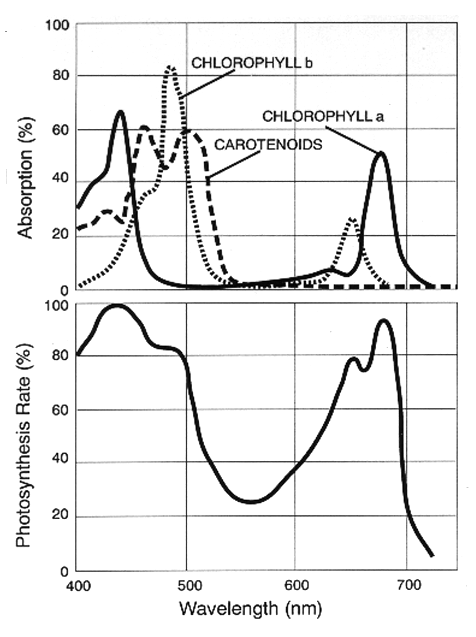
\includegraphics[width=0.5\textwidth]{figures/PAR_spectrum.png}
    \caption{The PAR Action Spectrum}
    \label{fig:PAR_spectrum}
\end{figure}

We can also define the productivity of an ecosystem with the \textbf{Gross Primary Productivity} (GPP) and the \textbf{Net
Primary Productivity} (NPP). GPP is the total amount of carbon fixed by photosynthesis in an ecosystem per unit time,
whereas NPP is the GPP minus the amount of carbon released by respiration i.e. $NPP = GPP - R$.

Around 50\% of the GPP is used for respiration, the other 50\% is used for growth.

\subsubsection{The Terrestrial Biosphere as a Carbon Source and Sink}
\label{sec:terrestrial-carbon-source-sink}

As noted in section \ref{sec:carbon-cycle}, the terrestrial biosphere is a sink for \COtwo, both from natural and
anthropogenic origin. Natural variability of the terrestrial biosphere occurs and can perturb the magnitude of this
sink. 

However, anthropogenic activity has a significant impact. Indeed, land use and change through deforestation and some
agricultural practices have resulted in the terrestrial biosphere becoming a net source of \COtwo in some regions
(e.g. the tropics). On the contrary, in other regions this is in fact the opposite, where afforestation and reforestation
have resulted in the terrestrial biosphere becoming a net sink of \COtwo and some regions even have net negative land
carbon emissions.

It is important the permanence of the carbon sink is considered when thinking about the influence of the terrestrial
biosphere on atmospheric \COtwo concentrations. For example, wildfires can perturb concentrations, but vegetation
tends to regrow and reabsorb the \COtwo released, meaning this is a transitory effect.

\subsubsection{Climate-Carbon Feedbacks}
\label{sec:climate-carbon-feedbacks}

Both photosynthesis and respiration are temperature dependent. As such changes to the climate will perturb the terrestrial
carbon cycle and therefore the atmospheric \COtwo concentration. Some of these feedbacks follow:

\begin{itemize}
    \item `Greening' of the Earth due to the \textbf{CO\textsubscript{2} Fertilisation Effect}: This is the increase in
    photosynthesis due to the increase in \COtwo concentration in the atmosphere. This is a negative feedback as the
    increase in photosynthesis will result in a decrease in atmospheric \COtwo concentration, which will in turn result
    in a decrease in photosynthesis. This enhances the land carbon sink.
    \item Relaxation on factors limiting plant growth - water, sunlight availability and temperature.
    \item Increase in respiration due to the increase in temperature. This is a positive feedback as the increase in
    respiration will result in an increase in atmospheric \COtwo concentration, which will in turn result in an increase
    in temperature which leads to even more respiration. This limitex the land carbon sink.
\end{itemize}

The impact of these is non-trivial and is still an area of active research.

\subsection{The Oceanic Carbon Cycle}
\label{sec:oceanic-carbon-cycle}

The ocean is a large carbon sink for atmospheric \COtwo. It takes up \COtwo through the dissolution of \COtwo in the
surface ocean and transforms it into \textbf{Dissolved Inorganic Carbon} (DIC). We can define DIC as:

\begin{align}
\text{DIC} &= \text{Dissolved Carbon Dioxide} + \text{Carbonic Acid} + \text{Bicarbonate} + \text{Carbonate} \nonumber \\
\text{DIC} &= \text{CO\textsubscript{2 (aq)}} + \text{H\textsubscript{2}CO\textsubscript{3}} 
+ \text{HCO\textsubscript{3}\textsuperscript{-}} + \text{CO\textsubscript{3}\textsuperscript{2-}} \nonumber
\end{align}


As we can expect, DIC has increased over the last few decades due to the increase in anthropogenic \COtwo emissions.
As per teh equation above we can see that this increase in DIC leads to a decrease in pH, i.e. ocean adification. This 
is partially buffered but oceanic adification is still a an occurrence and therefore a concern.

\subsubsection{Controls on Oceanic Carbon Uptake}
\label{sec:controls-oceanic-carbon-uptake}

How much the oceans are able to absorbe \COtwo is dependent on two main factors: atmospheric \COtwo concentration and
oceanic temperature:
\begin{itemize}
    \item Oceans are able to absorb more \COtwo as DIC when atmospheric \COtwo concentration is higher. However, the 
    rise between atmospheric \COtwo concentration and DIC is not linear, meaning the oceans' ability to keep absorbing
    \COtwo as concentrations increase more and more is reducing.
    \item Oceans are able to absorb more \COtwo as DIC when oceanic temperature is lower. This is because the solubility
    of \COtwo in water is higher at lower temperatures. It therefore follows that increasing oceanic temperature reduces
    the oceans' ability to act as carbon sinks.
\end{itemize}

\subsubsection{The Ocean Biological Carbon Pump}
\label{sec:ocean-biological-carbon-pump}

This is the process by which carbon is transported from the surface ocean to the deep ocean. It is a biological process
where the transformation of DIC into organic carbon occurs through photosynthesis of marine plants and phytoplankton. 
These living organisms then die and sink to the deap ocean. During this process, some of the organic carbon will decompose
and be released back into the ocean as DIC. However, some of it will be buried in the deep ocean, which is a carbon sink.

The remineralisation depth, or the depth at which 63\% of the organic carbon has been remineralised determines the time 
interval until the carbon is released back into the atmosphere. A shallower depth will reduce the capacity fo the ocean
to draw down anthropogenic carbon emissions.



\newpage
\section{Other Climate Forcers}
\label{sec:other-climate-forcers}

\subsection{Well-Mixed Greenhouse Gases}
\label{sec:well-mixed-greenhouse-gases}

We have seen in previous sections that carbon dioxide is the main forcing agent of anthropogenic climate change, however,
there are severall other important players. These are are a variety of gases that are grouped into what is called the
\textbf{well-mixed greenhouse gases} (WMGHG). These are gases that are well-mixed in the atmosphere (troposphere), i.e. 
their concentrations do not vary significantly with grographical location or height. The main WMGHG are methane, CFC-11
and CFC-12.\\

Methane is the second most important anthropogenic greenhouse gas. It is emitted from a variety of sources, both natural
and anthropogenic. Its atmospheric lifetime is $\sim$12 years and it is removed from the atmosphere by reaction with the
\ce{OH} radical. Its concentration rate increase is of $\sim$18Tg\ \ce{CH4}yr$^{-1}$, i.e. emissions increase by $\sim$10\%
per decade (has been for the past two decades).\\

CFC-11 and CFC-12 are \textbf{chlorofluorocarbons} (CFCs) and are synthetic gases, part of the family of Halocarbons
(hydrocarbons that have had some or all of their hydrogen atoms replaced by halogen atoms). They are emitted from
anthropogenic sources and have lifetimes of $\sim$50 and $\sim$100 years for CFC-11 and CFC-12 respectively. 

\noindent These are inert in the troposphere but dissociate in the stratosphere leading to ozone depletion. Environmental and 
health concerns have led to the Montreal Protocol in 1987 ultimately prohibited CFC production by 2000 leading to a
decrease in their atmospheric concentrations.

\subsection{Aerosol Radiative Forcing}
\label{sec:aerosol-radiative-forcing}

Aerosols are small liquid drops or particulates suspended in the atmosphere. They can be natural or anthropogenic in
origin and can be made up of many different constituents. They can be emitted directly into the atmosphere (primary) or
formed in the atmosphere as a result of chemical processes (secondary).\\

Aerosols have a direct effect on the climate by scattering and absorbing radiation. They also have an indirect
effect by modifying the properties of clouds.

Some aerosols like black carbon or soot have a predominantly warming effect since they absorb radiation thus causing
them to warm up. More commonly, aerosols have a predominantly cooling effect since they scatter radiation back to space,
examples of this are sulphate aerosols and sea salt aerosols. It is for this reason that aerosols are believeed to have
had a cooling effect on the climate for the past 250 years or so.\\

Some aerosols like sulphate aerosols can also act as \textbf{cloud condensation nuclei} (CCN) and thus modify the 
properties of clouds. If more aerosols are present, then more CCN are present and thus more cloud droplets are formed
(smaller droplets) and thus the cloud is brighter and more reflective. This is known as the \textbf{first aerosol
indirect effect} or \textbf{Twomey effect}. 

Other indirect effects link aerosol to changes in precipitation. The smaller droplets seen above take longer to grow into
raindrops, delaying precipitation and prolonging the cloud lifetime. Both of these effects are believed to have a
cooling effect on the climate.

\begin{figure}[h]
    \centering
    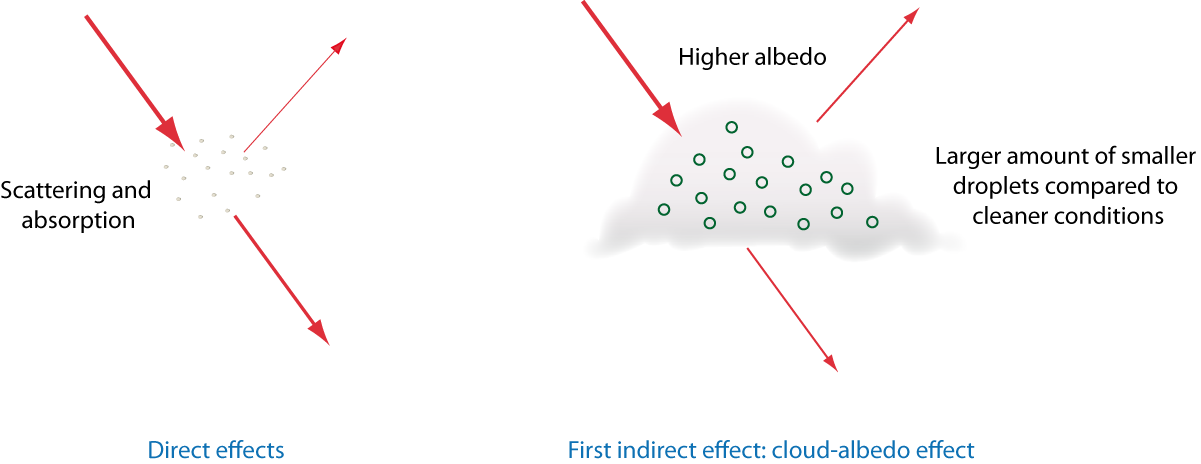
\includegraphics[width=0.8\textwidth]{figures/aerosol.png}
    \caption{Direct and indirect effects of aerosols on the climate.}
    \label{fig:aerosol}
\end{figure}

\subsection{Comparing the Impact of Different Forcing Agents}
\label{sec:comp-impact-diff}

To determine the impact a forcing agent (radiative gas or aerosol) has on the climate, we need to consider two more
things:
\begin{itemize}
    \item The lifetime of the forcing agent in the atmosphere.
    \item The radiative efficiency of the forcing agent, i.e. the ability of the forcing agent to cause a change in
    radiative forcing per unit change in concentration or amount thereof.
\end{itemize}

Hence the difficulty to compare the impact of different forcing agents without some deeper analysis. 

A metric that procides a means to compare the effectiveness of different agents to that of \ce{CO2} is the 
\textbf{Global Warming Potential} (\hyperlink{glo:global_warming_potential}{GWP}). We can define it as:
$$
\text{\hyperlink{glo:global_warming_potential}{GWP}} = \frac{\int_0^{\text{TH}} a_x[C_x(t)]dt}{\int_0^{\text{TH}} 
a_r[C_r(t)]dt}
$$
where $a_x$ is the radiative efficiency of the forcing agent $x$, $C_x(t)$ is the time-dependent concentration (decay)
of the forcing agent $x$, $a_r$ is the radiative efficiency of the reference gas (\ce{CO2}), $C_r(t)$ is the
time-dependent concentration (decay) of the reference gas (\ce{CO2}) and TH is the time horizon, or length of time over
which we evalueate the impact of the agent relative to the reference. Using \ce{CO2} as the reference gas is simply a
convention.

\begin{tcolorbox}
    \textbf{Example: Methane}\\
    We assume that we have an initial concentration of methane $C_0$ that decays exponentially with time (assumption). 
    We say that after time $\tau$ the concentration of methane has decreased by a factor of $e$ (63\%). We can then 
    caluculate the absolute GWP for methane (the numerator in the equation above) as:
    $$
    \text{AGWP}_x = \int_0^{\text{TH}} a_x[C_x(t)]dt = a_x C_{0x}\int_0^{\text{TH}} [e^{-t/\tau}]dt = 
    a_xC_{0x}\tau(1-e^{-\text{TH}/\tau})
    $$

    We note that \ce{CH4} has a radiative efficiency by \textbf{mass} of $\sim$72x that of \ce{CO2} so we write that
    $$
    a_xC_{0x} \approx 72a_rC_{0r}
    $$
    and \ce{CH4} lifetime is $\sim$12 years compared to \ce{CO2} lifetime of $\sim$200 years so we can write that the 
    global warming potential for methane is:
    $$
    \text{\hyperlink{glo:global_warming_potential}{GWP}}_{\text{CH4}} = 72\ \frac{12\left[1-e^{-\text{TH}/12}\right]}
    {200\left[1-e^{-\text{TH}/200}\right]}
    $$

    For reference we can see that in 20 years the GWP for methane is 37x that of \ce{CO2}, in 100 years it is 11x and
    500 years it is only 4.7x.
\end{tcolorbox}

This metric will be useful for policy makers to make a first order assessment of the climate impact of different
choices (e.g. changes to energy production, agricultural practices, etc.) on different timescales.


\newpage
\section{Climate Timescales and Sensitivity}
\label{sec:climate-timescales}

It is apparent that the climate system has some inertia and that the response to
an external forcing is not immediate.
In L7 a ``thought experiment'' is outlined where the Earth is initially assumed 
to be in equilibrium and then its \ce{CO2} concentration is doubled. In it we
see that, as a result of said \textbf{thermal inertia}, the Earth requires 
some time for it to reach a new equilibrium. In the following sections we will 
try to quantify how long it takes for this new equillibrium to be reached, i.e.
what is the \textbf{adjustment timescale}.

\subsection{The First Law of Thermodynamics Applied to the Climate System}
\label{sec:first-law-thermo}

We begin by writing the first law of Thermodynamics in terms of energy:
$$
dU = dQ + dW \quad \text{Energy}
$$
and we can rewrite this in terms of power ($\frac{d}{dt}$):
$$
\frac{dU}{dt} = \frac{dQ}{dt} + \frac{dW}{dt} \quad \text{Power}
$$
where $U$ is the internal energy of the system, $Q$ is the heat added to the system and $W$ is the work done \textbf{on}
the system (countrary to what we have seen in the Thermodynamics course).

We note all the variables are time dependent, so we can write for the control case and the perturbed (2x \ce{CO2}) case:
$$
\frac{dU_{CTL}(t)}{dt} = \frac{dQ_{CTL}(t)}{dt} + \cancel{\frac{dW_{CTL}(t)}{dt}} \quad \text{and} \quad 
\frac{dU_{P}(t)}{dt} = \frac{dQ_{P}(t)}{dt} + \cancel{\frac{dW_{P}(t)}{dt}}
$$
where the subscript $CTL$ denotes the control case and $P$ denotes the perturbed case. We also note that the work done
on/by the Earth is negligible.

Let us also define primed variables to be the differences between the perturbed and control cases, i.e.:
$$
U'(t) = U_{P}(t) - U_{CTL}(t) \quad \text{and} \quad Q'(t) = Q_{P}(t) - Q_{CTL}(t)
$$
it therefore follows from their definitions that
$$
\frac{dU'(t)}{dt} = \frac{dQ'(t)}{dt}.
$$

We write $\Delta Q_{ext}$ is the external (anthropogenic) forcing due to the 2x
increase in \ce{CO2} and $\Delta Q_{int}$ is the corresponding internal feedback
response. It then follows that at some given time $t$ the total heating on the
system (Earth) is the sum of both these terms ($\Delta Q_{ext} + \Delta Q_{int}$).
We can then write:
$$
\frac{dQ'(t)}{dt} = \left[\Delta Q_{ext}(t) + \Delta Q_{int}(t)\right] 4\pi 
\left(R_E + \cancel{z_{atm}}\right)^2 \quad \quad \because R_E \gg z_{atm}
$$ 
where $R_E$ is the radius of the Earth and $z_{atm}$ is the height of the
atmosphere, which is much smaller than $R_E$ and can therefore be neglected.

From equation \ref{eq:gamma} from section \ref{sec:forcing_feedback} we can
rewrite $\Delta Q_{int}(t)$ in terms of the feedback parameter:
$$
\Delta Q_{int}(t) = \gamma \Delta T_s(t) \quad \implies \quad \Delta T_s(t) = 
T_{s,P}(t) - T_{s,CTL}(t) = T_s'(t)
$$
and combining all of the above we can finally write:
$$
\boxed{\frac{dU'(t)}{dt} = \left(\Delta Q_{ext}(t) + \gamma \Delta T_s'(t)\right)
4\pi R_E^2}
$$

\noindent To proceed we will need some assumptions:
\begin{itemize}
    \item The only feedback process operating is blackbody feedback, i.e. we can
    rewrite $\gamma$ as $\gamma_{BB}$.
    \item The biospheric response is manifested in both oceans and land in for
    the sake of simplicity.
    \item Temperature change is constant throughout the atmosphere, i.e. assume
    no lapse rate change (see section \ref{sec:lapse_rate} for details on lapse
    rate).
    \item The atmosphere keeps a uniform surface temperature perturbation, i.e.
    surface temperature perturbation of the land and ocean are the same.
\end{itemize}

Recalling the definition of heat capacity $U = C \Delta T$, and using sensible 
values for these we can come up with rough estimates for how much energy the 
land, ocean and atmosphere can store provided we also have estimates for their 
mass. Lastly we can also consider the energy stored in the ice sheets, which is
in the form of latent heat. Let us write the following:
\begin{align}
    \Delta U_{atm}' &= m_{A}c_{A} \Delta T_{A}'(t) \nonumber \\
    \Delta U_{land}' &= m_{L}c_{L} \Delta T_{L}'(t) \nonumber \\
    \Delta U_{ocean}' &= m_{UO}c_{O} \Delta T_{UO}'(t) 
    + U_{DO}' \nonumber \\
    \Delta U_{ice}' &= l_fm_{ice}'(t) \nonumber
\end{align}

For detailed computation of the order of magnitude of these terms see L7 slides.
From there we will use the fact that heat capacity of the land and atmosphere is
about 2 orders of magnitude lower than that of the upper ocean ($10^{21}\ \text{vs}
\ 10^{23}$) for land/atmosphere vs ocean respecively. We can therefore neglect the 
former two terms. For the cryosphere, the order of magnitude is significant, its
calculation is covered on L7 slides, but we decide to ignore it due to reasons. 
We are therefore left with only the ocean term so 
we write:
$$
\boxed{
(Q_{ext} + \gamma_{BB} T_s') 4\pi R_E^2 \approx m_{UO}c_{O} \frac{dT_S'}{dt} + 
\frac{dU_{DO}'}{dt}} 
$$ \label{eq:energy_balance}

\subsection{Adjustment Timescale}
\label{sec:adjustment-timescale}

We will need to do some further derivation to reach the adjustment timescale. 
Let's begin by using the boxed equation \ref{eq:energy_balance} from the previous
section and introducing the concept of an `overturning' circulation strength, or
mass exchange rate $\Psi$ (mass/time) between the upper and deep ocean. We can 
then write:
$$
\frac{dU_{DO}'(t)}{dt} = \Psi c_O T_S'(t) - \Psi c_O T_{DO}'(t) = 
\Psi c_O (T_S'(t) - T_{DO}'(t))
$$
where a similar equation can be written for the upper ocean. With this newly
defined term and the original equation we can combine them to write:
$$
m_{UO}c_O \frac{dT_S'(t)}{dt} = 4 \pi R_E^2 \left(\Delta Q_{ext}(t) - 
\gamma_{BB} T_S'(t)\right) - \Psi c_O (T_S'(t) - T_{DO}'(t))
$$
and by defining $m_{UO} = A_0h_0\rho_0$ where $A_0$ is the surface area of the
ocean, $h_0$ is the depth of the upper ocean and $\rho_0$ is the density of the
upper ocean, and by dividing by area we can obtain a relation in terms of power
per unit area as follows:
$$
h_0 \rho_0 c_O \frac{dT_S'(t)}{dt} = \frac{4 \pi R_E^2}{A_0} \left(
\textcolor{red}{\Delta Q_{ext}(t)} - \textcolor{blue}{\gamma_{BB} T_S'(t)}\right)
- \textcolor{blue}{\frac{\Psi c_O}{A_0} (T_S'(t) - T_{DO}'(t))}
$$
where the term in \textcolor{red}{red} is the original forcing and the terms
in \textcolor{blue}{blue} are the damping of the change in surface temperature
(and therefore upper ocean internal energy) due to the blackbody feedback (first
blue term) and the heat exchange between the upper and deep ocean, i.e. oceanic
circulation (second blue term).\\

With this we can define $\eta$ as the ratio of the damping terms, i.e.:
$$
\eta = \frac{\Psi c_O}{4\pi R_E^2 \gamma_{BB}}
$$
so it follows that if $\eta \rightarrow 0$ then $\Psi \rightarrow 0$. This is
the weak oceanic circulation case.

\subsubsection{Weak Oceanic Circulation ($\eta \ll 1$)}
\label{sec:weak-oceanic-circulation}

In this case we can neglect the second blue term in the above equation and we
can write:
$$
\frac{dT_S'(t)}{dt} + \frac{4\pi R_E^2 \gamma_{BB}}{m_{UO}c_O} T_S'(t) = 
\frac{4\pi R_E^2 \Delta Q_{ext}(t)}{m_{UO}c_O}
$$
which is a first order linear differential equation (which we solve by using an
integrating factor). We also have some \textbf{initial conditions}: $T_S'(0) = 0$
since at $t=0$ the Earth is in equilibrium and there has not been any change in
temperature yet. The solution is then:
$$
\boxed{
T_S'(t) = \frac{\Delta Q_{EXT}}{\gamma_{BB}} \left(1-e^{t/t_a}\right)
}
$$
where, finally, we encounter the \textbf{adjustment timescale} $t_a$ which is
defined as:
$$
t_a = \frac{m_{UO}c_O}{4\pi R_E^2 \gamma_{BB}} \quad \implies \quad T_S'(t_a) =
\frac{\Delta Q_{EXT}}{\gamma_{BB}} \left(1-e^{-1}\right) \approx 0.63 
\frac{\Delta Q_{EXT}}{\gamma_{BB}} \approx \frac{2 \Delta Q_{EXT}}{3\gamma_{BB}}
$$
where the last approximation is the one given in the lectures.

It also follows that the equillibrium surface temperature ($T_{S,eq}'$) is reached
as time reaches $t_{eq}$ 
$$
\boxed{T_{S,eq}' = \frac{\Delta Q_{EXT}}{\gamma_{BB}}}
$$
which we can see in figure \ref{fig:surface_temp_weak}.

\begin{figure}[h]
    \centering
    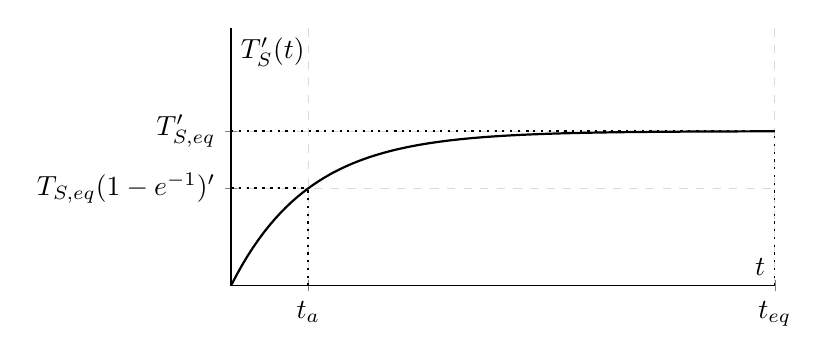
\begin{tikzpicture}
        \begin{axis}[
            xlabel=$t$,
            ylabel=$T_S'(t)$,
            xmin=0, xmax=7,
            ymin=0, ymax=5,
            xtick={0.994, 7},
            ytick={1.89, 3},
            yticklabels={$T_{S,eq} (1 - e^{-1})'$, $T_{S,eq}'$},
            xticklabels={$t_a$, $t_{eq}$},
            axis lines=middle,
            axis line style={-},
            width=0.7\textwidth,
            height=0.4\textwidth,
            grid=major,
            grid style={dashed, gray!30},
            % legend pos=north east,
            % legend style={font=\small, cells={align=left}},
            % legend cell align={left},
        ]
        \addplot[domain=0:7, black, thick,samples=100] {3*(1-exp(-x))};
        
        \addplot[domain=0:0.994, black, thick, dotted, samples=100] {3*0.63};
        \addplot[black, thick, dotted] coordinates {(0.994, 0) (0.994, 3*0.63)};
        % \node at (axis cs: 0.994, 3*0.63) [anchor=north west] {$T_{S,eq} (1-e^{-1})'$};
        % \node at (axis cs: 0.994, 0) [anchor=north] {$t_a$};

        \addplot[domain=0:7, black, thick, dotted, samples=100] {3};
        \addplot[black, thick, dotted] coordinates {(7, 0) (7, 3)};
        % \node at (axis cs: 3.5, 3) [anchor=south] {$T_{S,eq}'$};
        % \node at (axis cs: 7, 0) [anchor=north] {$t_{eq}$};

        \end{axis}
    \end{tikzpicture}
    \caption{Surface temperature change over time for the weak oceanic circulation}
    \label{fig:surface_temp_weak}
\end{figure}

\begin{tcolorbox}
    \textbf{Order-of-Magnitude Estimates:}\\
    We have expressions for $t_a$ and $T_{S,eq}'$ as follows:
    \begin{equation}
        t_a = \frac{m_{UO}c_O}{4\pi R_E^2 \gamma_{BB}} \quad \quad \text{and}
        \quad \quad T_{S,eq}' = \frac{\Delta Q_{EXT}}{\gamma_{BB}} \nonumber
    \end{equation}
    and we can use these to obtain some order-of-magnitude estimates. We use the
    following values:
    \begin{itemize}
        \item $m_{UO} = 3.4 \times 10^{19}\ \text{kg}$
        \item $c_O = 4.2 \times 10^3\ \text{J kg}^{-1} \text{K}^{-1}$
        \item $R_E = 6.4 \times 10^6\ \text{m}$
        \item $\gamma_{BB} = 4\epsilon' \sigma T_{S,eq}^3 \approx 3.8 
        \text{W m}^{-2} \text{K}^{-1}$
        \item $\Delta Q_{EXT} \approx 4\text{ W m}^{-2}$
    \end{itemize}

    \noindent From which we obtain:
    \begin{equation}
        t_a \approx 2.3\ \text{years} \quad \quad \text{and}
        \quad \quad T_{S,eq}' \approx 1\ \text{K} \nonumber
    \end{equation}

\end{tcolorbox}

\subsubsection{Strong Oceanic Circulation ($\eta \gg 1$)}
\label{sec:strong-oceanic-circulation}

In this case the upper and lower oceanic layers are strongly coupled, so we say
that $T_{DO}'(t) \approx T_S'(t)$ and therefore the second blue term in the 
equation cancels out. Once again, the equation be comes a first order linear
DE:
$$
\frac{dT_S'(t)}{dt} + \frac{4\pi R_E^2 \gamma_{BB}}{(m_{UO} + m_{DO})c_O} T_S'(t)
= \frac{4\pi R_E^2 \Delta Q_{EXT}(t)}{(m_{UO} + m_{DO})c_O}
$$

The solution, just as before is exponsential and we can write for $t_a$:
$$
\boxed{t_a = \frac{(m_{UO} + m_{DO})c_O}{4\pi R_E^2 \gamma_{BB}} \approx 
\frac{m_{DO}c_O}{4\pi R_E^2 \gamma_{BB}}} \quad \sim 100\text{s years}
$$

So we can see that the interaction between the upper and lower oceanic layers
has a significant effect on the adjustment timescale, i.e. it is a significant
damping factor on the rate of change of $T_S'(t)$. This is shown in figure
\ref{fig:surface_temp_timescale}.


\begin{figure}[h!]
    \centering
    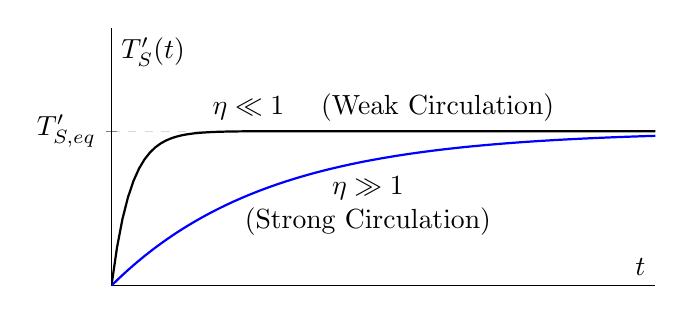
\begin{tikzpicture}
        \begin{axis}[
            xlabel=$t$,
            ylabel=$T_S'(t)$,
            xmin=0, xmax=7,
            ymin=0, ymax=5,
            xtick={0},
            ytick={3},
            yticklabels={$T_{S,eq}'$},
            xticklabels={},
            axis lines=middle,
            axis line style={-},
            width=0.7\textwidth,
            height=0.4\textwidth,
            grid=major,
            grid style={dashed, gray!30},
            legend pos=north east,
            legend style={font=\small, cells={align=left}},
            legend cell align={left},
        ]
        \addplot[domain=0:7, black, thick, samples=100] {3*(1-exp(-4*x))};
        \node at (axis cs: 3.5, 3) [anchor=south] 
        {$\eta \ll 1 \quad$ (Weak Circulation)};

        \addplot[domain=0:7, blue, thick, samples=100] {3*(1-exp(-0.5*x))};
        \node at (axis cs: 3.3, 2.3) [anchor=north, align=center] 
        {$\eta \gg 1$\\(Strong Circulation)};

        \end{axis}
    \end{tikzpicture}
    \caption{Strong vs weak oceanic circulation surface temperature change over time}
    \label{fig:surface_temp_timescale}
\end{figure}

\subsection{Climate Sensitivity}
\label{sec:climate-sensitivity}

In the section above (section \ref{sec:adjustment-timescale}) we have assumed a
number of things, some of which were not entirely realistic. 

One such assumption was the fact that no feedbacks other than blackbody feedback
were operating. We therefore used $\gamma_{BB}$ as the feedback parameter but in
fact we know that $\gamma = -\gamma_{BB} + \gamma_{\ce{H2O}} + 
\gamma_{\text{Albedo}} + \dots$ so we must rethink our model.We have seen that
$t_a \propto \frac{1}{\gamma}$ so it follows that changing $\gamma$ will change
the adjustment time $t_a$.\\

We define the \textbf{climate sensitivity} as the equillibrium global mean surface
temperature change in response to a doubling of \ce{CO2} concentration, i.e.
the previously seen $T_{S,eq}'$. To improve upon the previous blackbody-only
model, we can define the \textbf{net feedback parameter} $f$ as follows:
$$
f = \frac{\gamma_{\ce{H2O}} + \gamma_{\text{Albedo}} + \gamma_{\text{Clouds}} + 
\dots}{\gamma_{BB}} = \sum_i \frac{\gamma_i}{\gamma_{BB}}
$$
where $\gamma_i$ is the feedback parameter due to the $i$-th feedback process 
we wish to account for. We can now rewrite the climate sensitivity ($T_{S,eq}'$)
in terms of $f$ as follows:
$$
T_{S,eq}' = \frac{\Delta Q_{EXT}}{\gamma_{BB}} = \boxed{\frac{\Delta Q_{EXT}}{
\gamma_{BB} (1 - f)}}
$$
such that we now only have to consider the net feedback parameter $f$ to gain
insight into the \textbf{stability} of the climate system.\\

The following for some values of $f$ follow:
\begin{itemize}
    \item For negative values of $f$ (i.e. $f < 0$) the initial forcing $\Delta
    Q_{EXT}$ is dampened such that the adjustment time reduces and the equillibrium
    change in surface temperature is reduced. I.e. the equillibrium temperature
    is still higher than the initial temperature (because the 2x increase in \ce{CO2})
    is still present, but with a negative $f$ this increase in temperature is less
    than would be expected from the blackbody-only model.
    \item For $f = 0$ we essentially have the blackbody-only model.
    \item For positive values of $f$ (i.e. $f > 0$) the initial forcing $\Delta
    Q_{EXT}$ is amplified such that the adjustment time increases and the equillibrium
    change in surface temperature is increased. 
\end{itemize}

Finally, we notice that a value of $f = 1$ would mean that the climate system
is unable to reach an equillibrium, i.e. the planet is unable to ever radiate 
enough energy to space to counteract the effect of the original forcing and all
the operating feedbacks. This is called a \textbf{runaway greenhouse effect}.


\newpage
\section{Observing Our Climate}
\label{sec:observing_climate}

As we have seen in previous sections, signals of climate change are quite small
in section \ref{sec:climate-timescales} we see that a 2x in \ce{CO2} concentration
``only'' leads to a few degrees temperature difference. It is of very high 
importance therefore to be able to measure these changes 
\hyperlink{glo:accuracy}{accurately} and \hyperlink{glo:precision}{precisely} 
(see glossary for definitions) as to be able to detect anthropogenic signals
and distinguish them from \textbf{natural variability}.\\

\subsection{Examples of Potential Issues: In-Situ and Ground Based Measurements}
\label{sec:issues}

\subsubsection{The Urban Heat Island Effect}
\label{sec:uhi}

\begin{figure}[h]
    \centering
    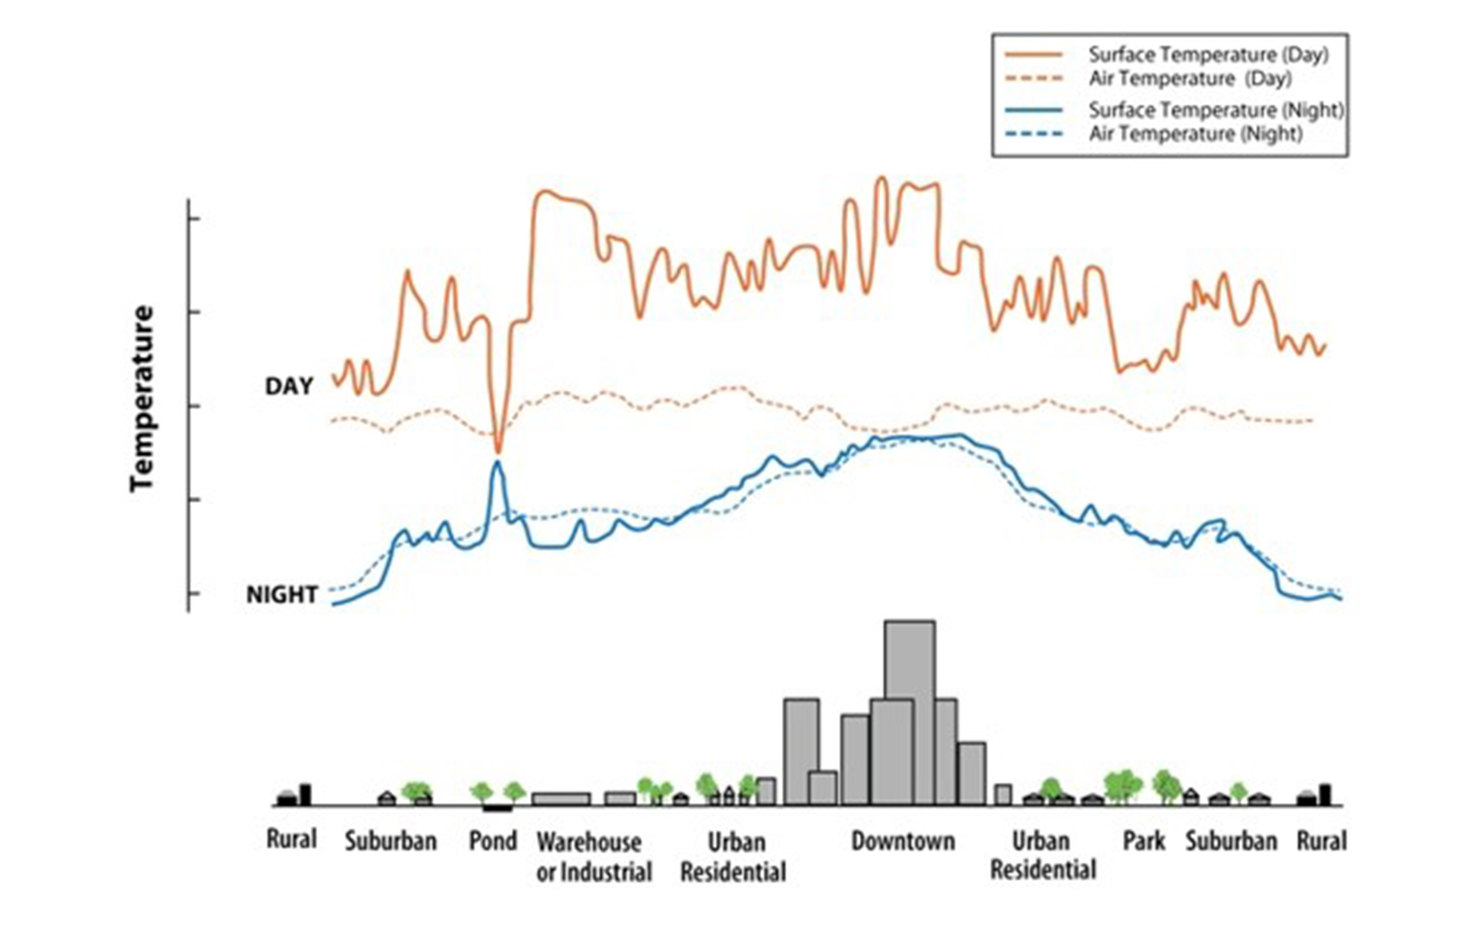
\includegraphics[width=0.65\textwidth]{figures/urban_heat_island.jpeg}
    \caption{Urban Heat Island Effect.}
    \label{fig:uhi}
\end{figure}

Figure \ref{fig:uhi} shows a schematic of the \textbf{urban heat island effect}.
This is a phenomenon where urban areas are warmer than their rural surroundings.
This is especially true at night. Some reasons for this are:
\begin{itemize}
    \item \textbf{Albedo}: Urban areas have a lower albedo than rural areas. 
    This means that they absorb more \gls{SW} radiation and therefore heat up 
    more. This is obvious when we consider that some key urban materials like 
    asphalt have an albedo much lower of that of vegetation.
    \item \textbf{Thermal Inertia}: Urban areas have a lower thermal inertia than
    rural areas. This means that they heat up more quickly during the day and cool
    down more quickly during the night. The fact that they heat up more during
    the day means that they release more heat during the night, further Increasing
    temperatures at when the sun does not shine.
    \item \textbf{Anthropogenic Heat}: Urban areas have a higher concentration of
    anthropogenic heat sources (cars, air conditioning, heating, etc.) than rural areas.
    \item \textbf{Evapotranspiration}: Urban areas have a lower evapotranspiration
    rate than rural areas. This means that less energy is used to evaporate water
    and more energy is used to heat the air. This is the case due to the lack of
    vegetation and bodies of water (ponds, lakes, etc.) in urban areas.
\end{itemize}

We can define the \textbf{Urban Heat Island Index} (somehow abbreviated UHI) as
the maximum temperature difference between the urban and rural areas as a function
of time:
$$
\boxed{
\text{UHI}(t) = \max(T_{\text{urban}}(t) - T_{\text{rural}}(t))
}
$$
which as previously mentioned is usually larger at night. In fact during the day
it is only usually the air that is closest to the ground that is different. We 
can also consider the following \textbf{surface energy balance}:
$$
(R_S^{\downarrow} - R_S^{\uparrow}) + (R_L^{\downarrow} - R_L^{\uparrow}) = H + E + Q
$$
where the $R_S$ terms represent the net downward \gls{SW} radiation at the surface,
the $R_L$ terms represent the net downward \gls{LW} radiation at the surface, $H$
is the sensible heat flux\footnote{Sensible heat flux means that is heat that can be ``sensed'',
or measured, usually with a thermometer. Latent heat flux in contrast cannot be
measured with a thermometer.}, $E$ is the latent heat flux and $Q$ is the ground heat 
transfer. It therefore follows that each of right hand side terms are affected 
due to urban characteristics.\\

It is therefore obvious that having measurement stations in/near urban areas will
lead to a bias in the measurements. This is a problem because most of the
\textbf{long term climate records} are based on measurements from urban areas.
Without corrections, warming trends would be amplified due to urbanisation.

\subsubsection{Changes in Sensor Design/Instrument Characteristics}
\label{sec:changes_in_sensor_design}

A clear example of how changes in how measurements are taken can lead to biases
in the data is the change in the design of \textbf{sea surface temperature} 
(\gls{SST}) measurements. There are a number of ways in which \gls{SST} measurements
can be taken including floating buoys, bucket measurements, hull contact sensors
and ship engine intake. It is clear, especially for the latter two measurement
methods, that the readings will have a bias. Such biased measurement techniques
are being phased out as we move towards more accurate and precise methods so 
once again it is crucial to make corrections when comparing new and old data.
See L9 for lower-level details.\\

Another example of this is the change in the design of global \textbf{radiosonde}
network. Radiosondes are instruments that are attached to weather balloons and
measure atmospheric parameters (temperature and humidity) as they ascend through
the atmosphere. The first measurements date back to the early 1900s so it is 
clear that the design of the instruments has changed significantly since then.
Furthermore, different regions of the world have used different typer of sensors
so once more it is crucial to make corrections when comparing new and old data 
and when comparing data from different regions when making a globally homogeneous
record.

Examples of what can cause discrepancies across different sensors include:
\begin{itemize}
    \item \textbf{Time constant}: The time it takes for the sensor to reach a new
    temperature after a change in temperature. This arises due to the sensor's
    \gls{thermal_inertia}.
    \item \textbf{Material composition}: Different materials have different
    \gls{emissivity} and \gls{absorptivity} characteristics, meaning that they
    will absorb and emit different amounts of radiation.
    \item \textbf{Sensor location}: The length of the string attaching the sensor
    to the balloon can affect the readings. This is because the balloons tend to
    have warmer temperatures than the environment around them.
\end{itemize}

\subsection{Surface Temperature Trends and the Impact of Satellite Observations}
\label{sec:surface_temp_trends}

Despite the issues mentioned above, after applying the necessary corrections,
we can still se a warming trend of about 1K over the last 100 years and this 
warming is more accentuated over land than over the oceans as per section 
\ref{sec:climate-timescales}.\\

Satellite observations have become a standard practice since the late 1970s for 
gathering data on the state of the atmosphere and surface, including 
temperature and humidity. These observations offer significant advancements over
traditional surface and in-situ measurements, evident in their higher spatial 
resolution and the availability of a more comprehensive and global sea-surface 
temperature (\gls{SST}) record starting from the late 1970s.

\subsection{Space-Based Observations}
\label{sec:space_based_obs}

In the previous section we outline some of the advantages of space-based
observations when compared to ``legacy'' means of climate observation. However,
space-based observations come with challenges and limitations of their own.\\

\noindent There are two main types of space-based sensors:
\begin{itemize}
    \item \textbf{Passive Sensors}: These sensors measure the \gls{LW} 
    radiation emitted by the Earth and backscattered light from the Sun. These
    are the most common type of sensors and have been used since the beginning
    of the space-based observation era to measure surface and atmospheric
    temperature.\\
    These are low-power devices so they are able to scan large portions of the
    Earth.
    \item \textbf{Active Sensors}: These newer sensors emit their own radiation and
    measure the amount of radiation that is reflected back to them (LIDAR, RADAR).
    These kind of sensors are particularly good at measuring clouds and aerosols
    and their vertical structure.\\
    These are high-power devices so they are only able to scan small portions of
    the Earth at once.
\end{itemize}

\noindent The climate variable that a sensor is measuring will be dependent on 
the wavelength examined by it. Always remember that the only kind of interaction
between the Earth and a satellite will be through \textbf{photon exchange}.

Up to now we have mostly considered \textbf{irradiance} $I_\lambda$: the amount
of energy per unit area per unit wavelength emitted or recieved from all directions
such that at the \gls{TOA} we have:
$$
\text{\gls{OLR}} = \int I_\lambda \text{d}\lambda
$$
but most satellite sensors measure \textbf{radiance} $L_\lambda$: the amount of
energy per unit area per unit wavelength per unit solid angle recieved from a
particular direction. Newer satellites are able to measure radiance in multiple
directions. Furthermore, it follows that if we are interested in these instruments
giving us insight into the temperature of the surface or the atmosphere that 
the light captured by these must be in the \gls{LW} part of the spectrum.

\begin{tcolorbox}
    \textbf{Aside on Radiance vs Irradiance}:\\

    Let's consider an observational instrument in space aimed at Earth, designed
    to measure Earth's reflected and emitted energy.\\

    \noindent \textbf{Irradiance}:

    Suppose the instrument is equipped with a sensor that measures the total 
    power incident on it per unit area from Earth, integrating over the entire
    field of view. This sensor does not differentiate between the various regions
    on Earth's surface it's viewing - it's simply recording the total power from
    all these regions per unit area. The measured quantity is the irradiance at 
    the sensor's location, arising from the totality of the Earth scene within 
    its field of view.\\

    \noindent \textbf{Radiance}:

    Now, consider a different instrument on the same platform, but this one is a
    hyperspectral imaging device - a bit like a camera sensor that can capture
    many different wavelengths and has many pixels. 
    This instrument is designed to measure the
    power received in each of its pixels per unit area per unit solid angle. 
    Each pixel corresponds to a specific area on Earth's surface, and the 
    instrument measures the power coming from that specific area and direction. 
    For each pixel, it quantifies the power received in each of a multitude of 
    narrow spectral bands, thereby providing a spectrum for each pixel.\\

    The quantity it measures is radiance. It is a directional quantity, 
    associated with a specific location (the corresponding surface area) and a 
    specific direction (the direction from that area to the instrument). \\

    For a given location on Earth's surface, the radiance varies with the direction.
    For example, if the location is a forest, the radiance in the direction of the 
    sun may be quite different from the radiance in a direction away from the sun, 
    due to the scattering properties of the trees. \\

    Therefore, while irradiance gives a measure of the total power per unit area
    received from all directions, radiance provides a detailed picture of the 
    power per unit area received from each specific direction. This allows for
    a more nuanced understanding of how light interacts with Earth's surface 
    and atmosphere.
\end{tcolorbox}


\subsection{Obtaining Temperature Information from Space and Schwarzschild's 
Equation}
\label{sec:schwarzschild}

To obtain temperature information from space we need to consider the following:
\begin{itemize}
    \item The interaction between the Earth's emmited \gls{LW} radiation and the
    atmosphere.
    \item How to describe these interactions mathematically.
    \item Translate this to temperature measurements from space.
\end{itemize}

\subsubsection{Interaction Between LW Radiation and the Atmosphere}
\label{sec:lw_atm}

There are three main ways in which \gls{LW} radiation interacts with the 
atmosphere: \textbf{absorption}, \textbf{emission} and 
\cancel{\textbf{scattering}}. We can neglect scattering in the \gls{LW} in times
of clear-sky conditions. This is not the case if there are clouds, but in such a
case we cannot measure the surface temperature anyway.\\

We can begin by considering absorption by a layer of atmosphere $dz$. As per the
\gls{beer_lambert}, we have the following:
$$
dL_{\lambda \text{abs}} = -L_\lambda \rho_{\text{a}} \kappa_\lambda^{\text{a}} dz
$$
where $dL_{\lambda \text{abs}}$ is the change in radiance due to absorption,
$L_\lambda$ is the incident radiance at the base, $\rho_{\text{a}}$ is the density
of the absorbing material and $\kappa_\lambda^{\text{a}}$ is the mass absorption 
coefficient.\\

Secondly, we consider the emission by a similar layer of atmosphere $dz$. As per
\gls{kirchoff} (\gls{LTE})we have the following:
$$
dL_{\lambda \text{em}} = B_\lambda(T_z) \rho_{\text{a}} \kappa_\lambda^{\text{a}} dz
$$
where $dL_{\lambda \text{em}}$ is the radience emmited by the layer, $B_\lambda(T_z)$
is the \textbf{Plank Function} at the temperature of the layer $T_z$ and
$\rho_{\text{a}} \kappa_\lambda^{\text{a}}$ is the \gls{emissivity} (equal to the
\gls{absorptivity}).

We can combine these two equations to obtain the following:
$$
dL_{\lambda} = -[L_\lambda + B_\lambda(T_z)] \rho_{\text{a}} 
\kappa_\lambda^{\text{a}} dz
$$
and bring in the concept of \hyperlink{glo:opticaldepth}{optical depth} 
$\tau_\lambda$ do do the following derivation:
\begin{gather*}
    \tau_\lambda = \int \rho_{\text{a}} \kappa_\lambda^{\text{a}} dz \quad 
    \implies \quad d\tau_\lambda = \rho_{\text{a}} \kappa_\lambda^{\text{a}} dz\\
    dL_{\lambda} = -[L_\lambda - B_\lambda(T_z)] \rho_{\text{a}} 
    \kappa_\lambda^{\text{a}} dz\\
    \frac{dL_{\lambda}}{d\tau_\lambda} + L_\lambda = B_\lambda(T_z)\\
\end{gather*}
which is a first order ODE that we can solve for $L_\lambda$ using an 
integrating factor and the following boundary conditions (see L10 for more 
details):
$$
\boxed{
\textcolor{orange}{L_\lambda(z_{\text{space}})} = 
\textcolor{blue}{L_\lambda(0)e^{-\tau_\lambda}} + 
\textcolor{red}{\int_0^{\tau_\lambda}B_\lambda(T_z) 
e^{-(\tau_\lambda - \tau_\lambda')} d\tau_\lambda'}}
$$

This is the \textbf{Schwarzschild Equation}. The term in \textcolor{orange}{orange}
is the radiance seen by the satellite, the term in \textcolor{blue}{blue} is the
radiance emitted by the surface that reaches the satellite despite the absorption
by the atmosphere and the term in \textcolor{red}{red} is the radiance emitted
by the atmosphere that reaches the satellite.

We can rewrite the above equation in terms of \textbf{\gls{transmissivity}} where
we use the following notation to write transmissivity of the atmosphere from 0
to $z_{\text{space}}$: $t_\lambda (0, z_{\text{space}}) = e^{-\tau_\lambda}$:
\begin{gather*}
    t_\lambda(z', z_{\text{space}}) = e^{-(\tau_\lambda - \tau_\lambda')} \quad
    \implies \quad \frac{dt_\lambda(z', z_{\text{space}})}{d\tau_\lambda'} =
    e^{-(\tau_\lambda - \tau_\lambda')}\\
\end{gather*}
and we obtain the Schwarzschild Equation in terms of transmissivity:
$$
\boxed{
    L_\lambda(z_{\text{space}}) = L_\lambda(0) t_\lambda(0, z_{\text{space}}) +
    \int_{t_\lambda(0, z_{\text{space}})}^1 B_\lambda(T_z) 
    dt_\lambda' (z', z_{\text{space}})
}
$$

Remember that we make the assumption that \textbf{the atmosphere is in \gls{LTE}}
and that there is \textbf{no scattering}.

\subsubsection{Weighting Functions}
\label{sec:weighting_functions}

When we attempt to retrieve temperature information from space, we will not use
the Schwarzschild Equation as written above, but rather we transform it into the
following in terms of altitude $z$:
$$
\boxed{
    L_\lambda(z_{\text{space}}) = L_\lambda(0) t_\lambda(0, z_{\text{space}}) +
    \int_{z=0}^{z_{\text{space}}} B_\lambda(T_z) \textcolor{red}{
    \frac{dt_\lambda' (z', z_{\text{space}})}{dz}} dz
}
$$
where the term in \textcolor{red}{red} is the \textbf{weighting function} 
$K_\lambda(z)$. Note that the weighting function could be defined in terms of 
any other variable so long as it is monotonic\footnote{Monotonic means that one
variable is either always increasing or always decreasing with respect to the
other variable. It also ensures that there is a one-to-one correspondence between 
variables. E.g. pressure and height.} with height.

The concept of a weighting function is a useful one because it allows us to
understand where from the atmosphere a particular wavelength is coming from as
measured by a satellite.

It follows that by scanning a number of different wavelengths we are able to 
obtain a vertical profile of the atmosphere for the particular feature we are 
interested in\footnote{This requires a constant gas density, so usually the \ce{CO2}
band is used} e.g. temperature, humidity, etc. Finally then, the higher the 
spectral resolution (i.e. the narrower the range of wavelengths the satellite
measures) the more vertical information the satellite can obtain.

\subsection{Issues With Satellite Based Records}
\label{sec:issues_satellite}

As with any other kind of measurement, satellite based measurements are not
without their own issues. Some of these include:
\begin{itemize}
    \item \textbf{Accuracy of Calibration}: Instruments must be callibrated 
    against a known reference or standard prior to launch to space as to convert
    a measurement to the required quantity. The \textbf{transfer of callibration}
    from ground to space is often unstable.
    \item \textbf{Length of Missions and Consistency of Instrumentation}: A 
    typical mission will last for about 3-5 years. This means that instruments 
    are replaced somewhat regularly, and although they are replaced with newer 
    and potentially slightly different equipment as to exploit new technologies,
    which can lead to inconsistencies in the data.
    \item \textbf{Orbit Decay}: The orbit of a satellite will decay over time
    due to atmospheric drag. This means that the satellite's altitude changes
    leading to changes in the measured signal.
    \item \textbf{Gaps in Data}: If launches are delayed, or if the satellite
    in orbit malfunctions and there are no others that can take over, then there
    will be gaps in the data.
    \item \textbf{Inversions}: Inversions are the process of transforming 
    satellite measurements into the required quantity. Like we have seen above,
    these inversions are ``models'' and as such have their limitations and 
    assumptions. It therefore follows that different models will yield different
    insight with the same data. (There is some extra detail in the last few 
    slides of L10, mainly examples).    
\end{itemize}



\newpage
\section{Modelling Our Climate}
\label{sec:climate-modelling}

Throughout the previous sections, we have discussed a number of climate models
with varying levels of complexity. They are all based on the fundamental
principle of energy conservation and equillibrium, i.e. energy input = energy
output for a planet in equillibrium, known as energy balance models (\gls{EBM}).
In this section we will have a look at some
of these models and explore different ways in which we can apply this principle 
to make more nuanced models.

\subsection{Energy Balance Models}
\label{sec:EBM}

\subsubsection{The Zero and One-Dimensional Energy Balance Models}
\label{sec:0D-1D-EBM}

The simplest energy balance model is the zero-dimensional energy balance model. 
We have covered this extensively in sections \ref{sec:introduction} and 
\ref{greenhouse_effect}. It is the model of photon energy exchange where the Earth
gets all its energy from the Sun and radiates it back into space (through albedo,
blackbody radiation etc.). 

Within this model we explored the \textbf{zero-layer} version, i.e. the no-atmosphere
model where we only account for the energy coming from the sun, 
\hyperlink{glo:albedo}{albedo} and blackbody radiation from the Earth's surface.
This was the energy balance equation:
$$
(1-\alpha) \text{\hyperlink{glo:TSI}{TSI}} = \sigma T_s^4
$$

Also in the aforementioned lectures is the \textbf{one-layer} version, i.e. the
atmosphere is treated as a single layer. In such a model we also account for the
\hyperlink{glo:emissivity}{emissivity} of the atmosphere and its 
\hyperlink{glo:absorptivity}{absorptivity} (which we stated are
equal in value for a system in \gls{LTE}). This was the energy balance equation:
$$
(1-\alpha) \text{\hyperlink{glo:TSI}{TSI}} = (1-\epsilon_a)\sigma T_s^4 + 
\epsilon_a\sigma T_a^4
$$
and it also lead to the introduction of the greenhouse effect. For more details 
see section \ref{greenhouse_effect}.\\

We can now extend this model to make it what is known as the \textbf{1-D \gls{EBM}}.
In this model we introduce latidudinal dependence. This is an obvious first choice
for independent variable since it is apparent that the energy balance is going 
to be different in the poles than in the equator.\footnote{We could also add
time-dependency, since it is apparent that this also has a significant effect}.
For now we will only consider the mean anual values for the energy balance, see
figure \ref{fig:1D-EBM}.

\begin{figure}[h]
    \centering
    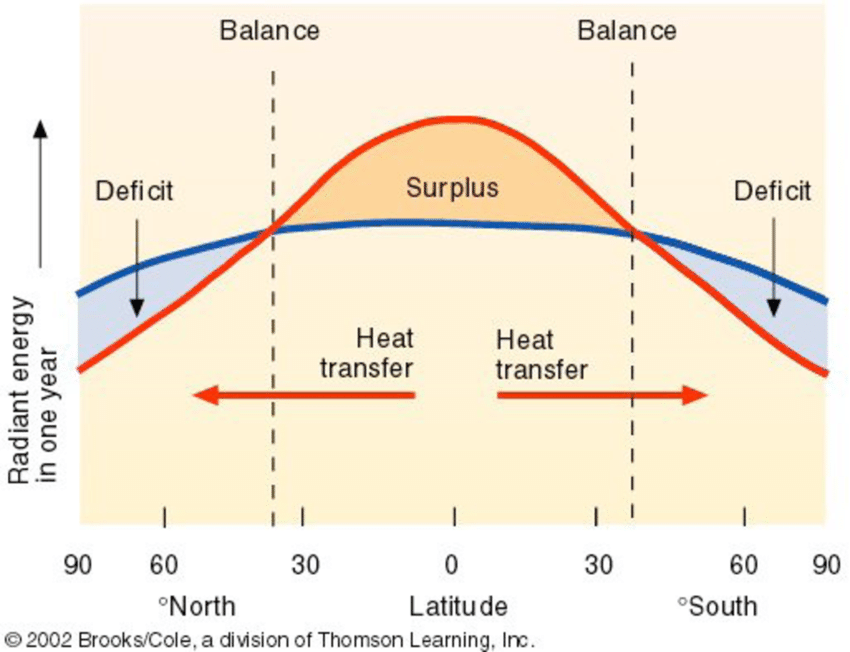
\includegraphics[width=0.6\textwidth]{figures/1debm.png}
    \caption{The 1-D Energy Balance Model. The energy balance is different in the
    poles than in the equator.}
    \label{fig:1D-EBM}
\end{figure}

As we see in figure \ref{fig:1D-EBM}, the energy balance is different in the
poles than it is in the equator (when averaged over the year). The relevance of 
this is that this will set the main circulation patterns of energy (both 
atmospheric and oceanic).

Let's express this model mathematically. We begin by writing the energy balance
equation:
$$
\frac{(1-\alpha)}{4} \text{\hyperlink{glo:TSI}{TSI}} = \epsilon'\sigma T_s^4
$$
where $\epsilon'$ is the effective emissivity of the Earth (see
\ref{sec:decompose_feedback}). It follows that for a perturbation from equillibrium
$$
C \frac{dT_s}{dt} = \frac{(1-\alpha)}{4} \text{\hyperlink{glo:TSI}{TSI}} - 
\epsilon'\sigma T_s^4
$$
where $C$ is the heat capacity per square meter. For a short range of values for
$T_s$ we can linearise as follows and substitute into the equation:
$$
\epsilon' \sigma T_s^4 \approx A + BT_s \quad \implies \quad C \frac{dT_s}{dt} 
\approx \frac{(1-\alpha)}{4} \text{\hyperlink{glo:TSI}{TSI}} - (A + BT_s)
$$
where $A$ and $B$ are constants. We can now ``slice'' the Earth into small 
latitudinal bands and consider the energy balance in each band $i$:
$$
C_i \frac{dT_{s,i}}{dt} \approx \frac{(1-\alpha_i)}{4} 
\text{\hyperlink{glo:TSI}{TSI}}_i - A - BT_{s,i}
$$
and finally we can include a term for the lateral heat transport ($F$) to complete
the model:
$$
C_i \frac{dT_{s,i}}{dt} + F(T_{s, i} - T_s) \approx \frac{(1-\alpha_i)}{4} 
\text{\hyperlink{glo:TSI}{TSI}}_i - A - BT_{s,i}
$$
where $F$ is in units of $Wm^{-2}K^{-1}$. The one-dimensional energy balance
model \textbf{must be solved numerically}.

\begin{figure}[h]
    \centering
    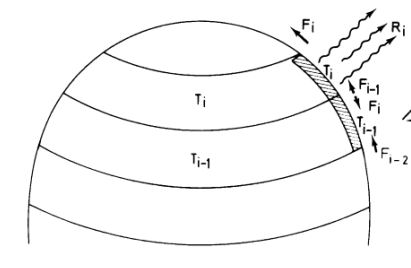
\includegraphics[width=0.4\textwidth]{figures/1demb diagram.png}
    \caption{Diagram of the 1D EMB.}
    \label{fig:1D-EBM-diagram}
\end{figure}

\subsubsection{Coupled General Circulation Models (CGCMs)}
\label{sec:CGCMs}

These are the most complex and complete models available, so called ``state-of-the-art''.
These are the kind of models used by the IPCC to make predictions about the future.
In the course we do not go too much into detail about these models, precisely due
to their complexity.\\

In these models, both the atmosphere and the ocean are divided into a grid of
boxes. The atmosphere is further divided into layers of altitude. These systems
are modelled as a set of coupled non-linear ordinary differential equations that
govern the evolution of the systems from a fluid dynamics perspective (in the 
atmosphere and ocean) while always ensuring conservation of momentum, mass and
energy.

Models have evolved significantly over time, with more and more layers of complexity
being added as computing power available increases and new inter-dependencies 
within the climate system are identified (i.e. the science evolves). Figure
\ref{fig:evolution-cgcm} shows the evolution of CGCMs over time with more components
being added as time goes on.

\begin{figure}[h]
    \centering
    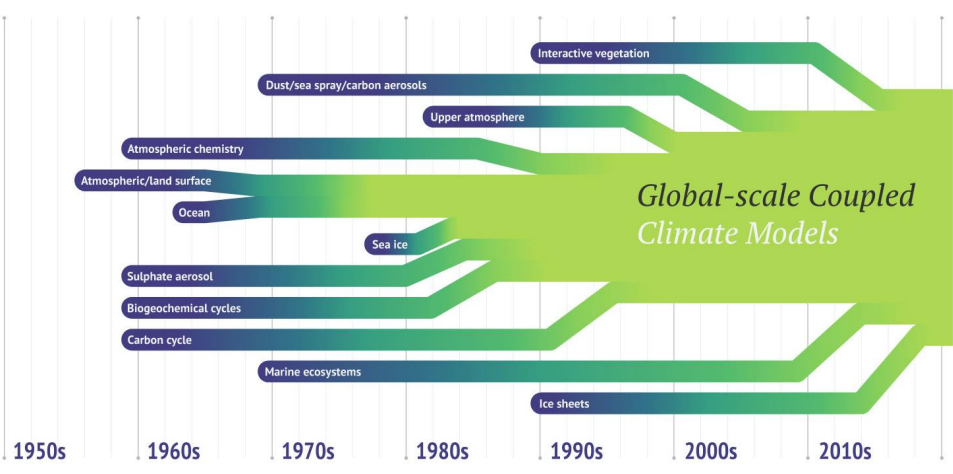
\includegraphics[width=0.75\textwidth]{figures/evolution cgcm.png}
    \caption{Evolution of CGCMs over time.}
    \label{fig:evolution-cgcm}
\end{figure}

\subsubsection{Earth System Models}
\label{sec:ESMs}

These are the absolute most advanced models available. They are essentially CGCMs
but not only simulate physical processes (oceans, land, atmosphere) but also
biogeochemical processes (most notably the carbon cycle) and the way they interact
with each other. This allows to introduce some additional feedbacks into the model
that are not present in CGCMs such as how warming may affect the ability of forests 
to absorb \ce{CO2}, or how changes in ocean circulation may alter the ocean's 
\ce{CO2} uptake.

\subsection{Model Parametrisation}
\label{sec:model-parametrisation}

In climate modelling, certain physical process cannot be modelled in a per-cell
basis due to their scale being too small, e.g. convection, cloud formation and
evolution and others. To model these, we use \textbf{parametrisation}.\\

In parametrisation, we find simplified 
representations or approximations of sub-grid phenomena, expressed in terms
of the larger-scale variables that the model does directly resolve. They are 
often based on empirical evidence from observations or more detailed process-based 
studies, or on theoretical understanding from physical laws. Within parametrisation
techniques we find two main types:\\

\textbf{Diagnostic Scheme}: A diagnostic scheme determines the outcome (e.g., 
the presence and properties of clouds) directly from the current state of the 
large-scale variables, with no memory of past states. In other words, given the 
same current state, a diagnostic scheme will always produce the same outcome.\\

\textbf{Prognostic Scheme}: A prognostic scheme is more advanced, it includes some 
form of temporal evolution or memory, meaning that the outcome can depend on past 
states as well as the current state. This allows the model to represent processes 
that have some inherent time-dependence or persistence, such as the life cycle of 
clouds or the accumulation of snow. Given the same current state, a prognostic 
scheme could produce different outcomes depending on the prior sequence of states.\\

\noindent The main idea to remember between the two is that prognostic schemes
have memory (time dependence) while diagnostic schemes do not.

Also worth remembering is that clouds are the main source of uncertainty in climate
models by far, analytical solutions become impossible so with every approximation
comes error (error in frequency of occurrence, error in amount and properties and
error in location and timing).

\subsection{Costs of Climate Modelling}
\label{sec:costs-climate-modelling}

Climate models are very expensive to run, both in terms of computing power and
time.
\begin{itemize}
    \item Atmosphere is the most expensive component of the model to run and is
    typically the bottle neck of climate models (radiation and chemistry schemes
    are very computationally intensive)
    \item Timestep in Earth System Model worlds is typically 20 minutes for
    dynamics and 1h for radiation
    \item 1 week of very high performance computer time yields about 40 years of
    simulated climate. When we consider that we want to simulate 1000 or 2000 years
    of climate per model, and include many of them in an ensemble for an IPCC report
    we can see how this becomes a very expensive and time consuming process.
    \item There is about 1 million `basic' variables only to model oceans and
    atmosphere. This is very memory consuming
\end{itemize}



\newpage
\section{Climate Policy and Implications}
\label{sec:climate_policy}

It is clear that there is an anthropogenic impac on the climate as per all of the
information presented in the previous sections. The question now is what can be done
about it such that humanity can continue to enjoy prosperity.\\

Precisely because anthropogenic climate change is believed to be a threat to said
prosperity, there has been international recognition of the need to implement 
policies to mitigate the effects and the scale of dangerous climate change. The 
most clear example of this is the 2015 Paris Agreement, which was signed by 200
countries and sets out the following goals:
\begin{itemize}
    \item To limit the increase in global surface temperature by \textless{}2K above 
    pre-industrial revolution levels by the end of 2100.
    \item To achieve ``net-zero'' emissions by the second half of the 21st century,
    allowing for carbon capture technology to be used to offset any remaining
    emissions.
    \item To set up a ``global stocktake'' to assess whether the goals are being
    met by individual countries. This is also called the \textbf{intended nationally
    determined contributions} (INDCs). The first such stocktake will be in 2023.
\end{itemize}

The Paris Agreement is complementary to the UN's 17 Sustainable Development Goals
(SDGs), which are a set of goals to be achieved by 2030. See Figure \ref{fig:SDGs}.

\begin{figure}[ht]
    \centering
    
\includegraphics[width=0.85\textwidth]{figures/sdg.jpeg}
    \caption{The 17 Sustainable Development Goals}
    \label{fig:SDGs}
\end{figure}

\subsection{How to Achieve the Climate Goals}
\label{sec:achieve_climate_goals}

The above goals are ambitious, so if we wish to achieve them we have to analyse
what the existing patterns of emissions are and how they need to be changed to
achieve the goals.

\begin{figure}[ht]
    \centering
    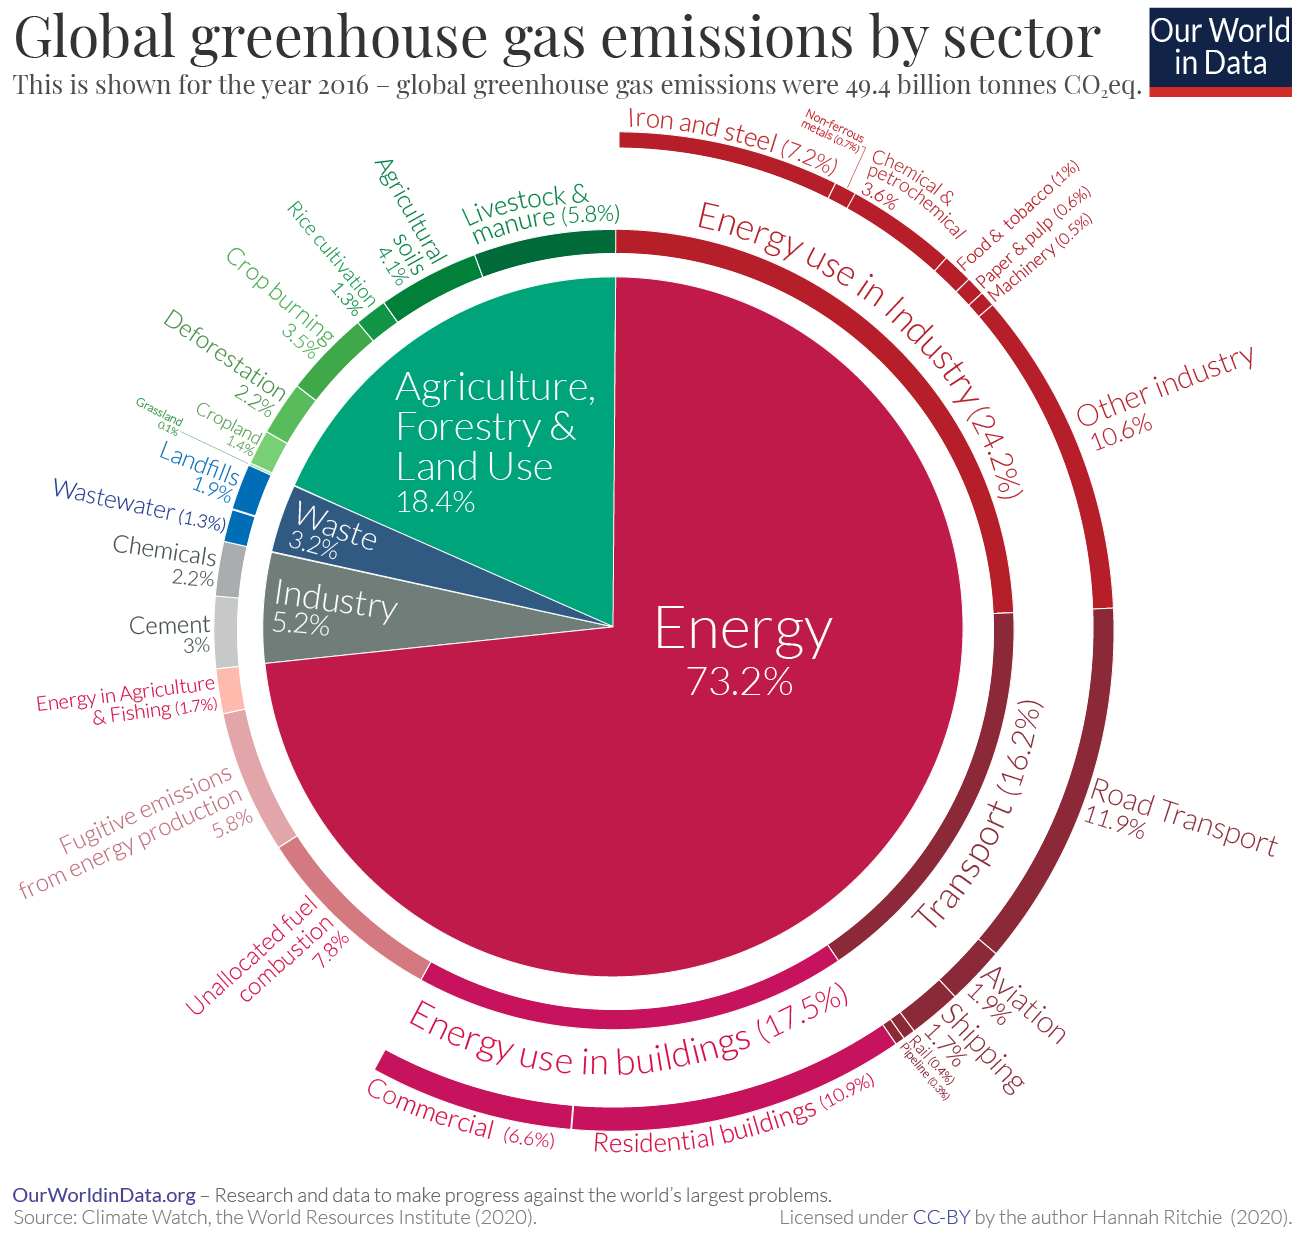
\includegraphics[width=0.55\textwidth]{figures/emissions-pie-chart.png}
    \caption{Global \ce{CO2} emissions by sector}
    \label{fig:emissions_pie_chart}
\end{figure}

Figure \ref{fig:emissions_pie_chart} shows us the breakdown of global \ce{CO2}
emissions by sector. We clearly see that if we wish to limit the anthropogenic
impact of climate change, we need to focus on the energy sector. \\

\noindent The \textbf{Kaya Identity} allows us to relate the total emissions to four key
factors: population, GDP per capita, energy intensity and carbon intensity:
\begin{equation*}
    \boxed{
    \begin{array}{c c c c c c c c c}
    \text{Total Emissions} & = & \text{Population} & \times & \text{GDP per capita}
    & \times & \text{Energy Intensity} & \times & \text{Carbon Intensity} \\
    \text{F\ (kg)} & = & \text{P} & \times & \text{GDPP (\$ pp)} &\times & \text{EI\ (kWh/\$)}
    & \times & \text{CI\ (kg/kWh)}\\
    \end{array}}
\end{equation*}

We see that in the past decades the increase in emissions (F) is largely due to 
the population increase as well as the increase in GDP per capita. By contrast, 
the energy intensity and carbon intensity have decreased, though to a smaller
extent. See Figure \ref{fig:kaya_components}. We also note that these individual
factors change from country to country (for more details see L12 slides 9 onwards).

\begin{figure}[ht]
    \centering
    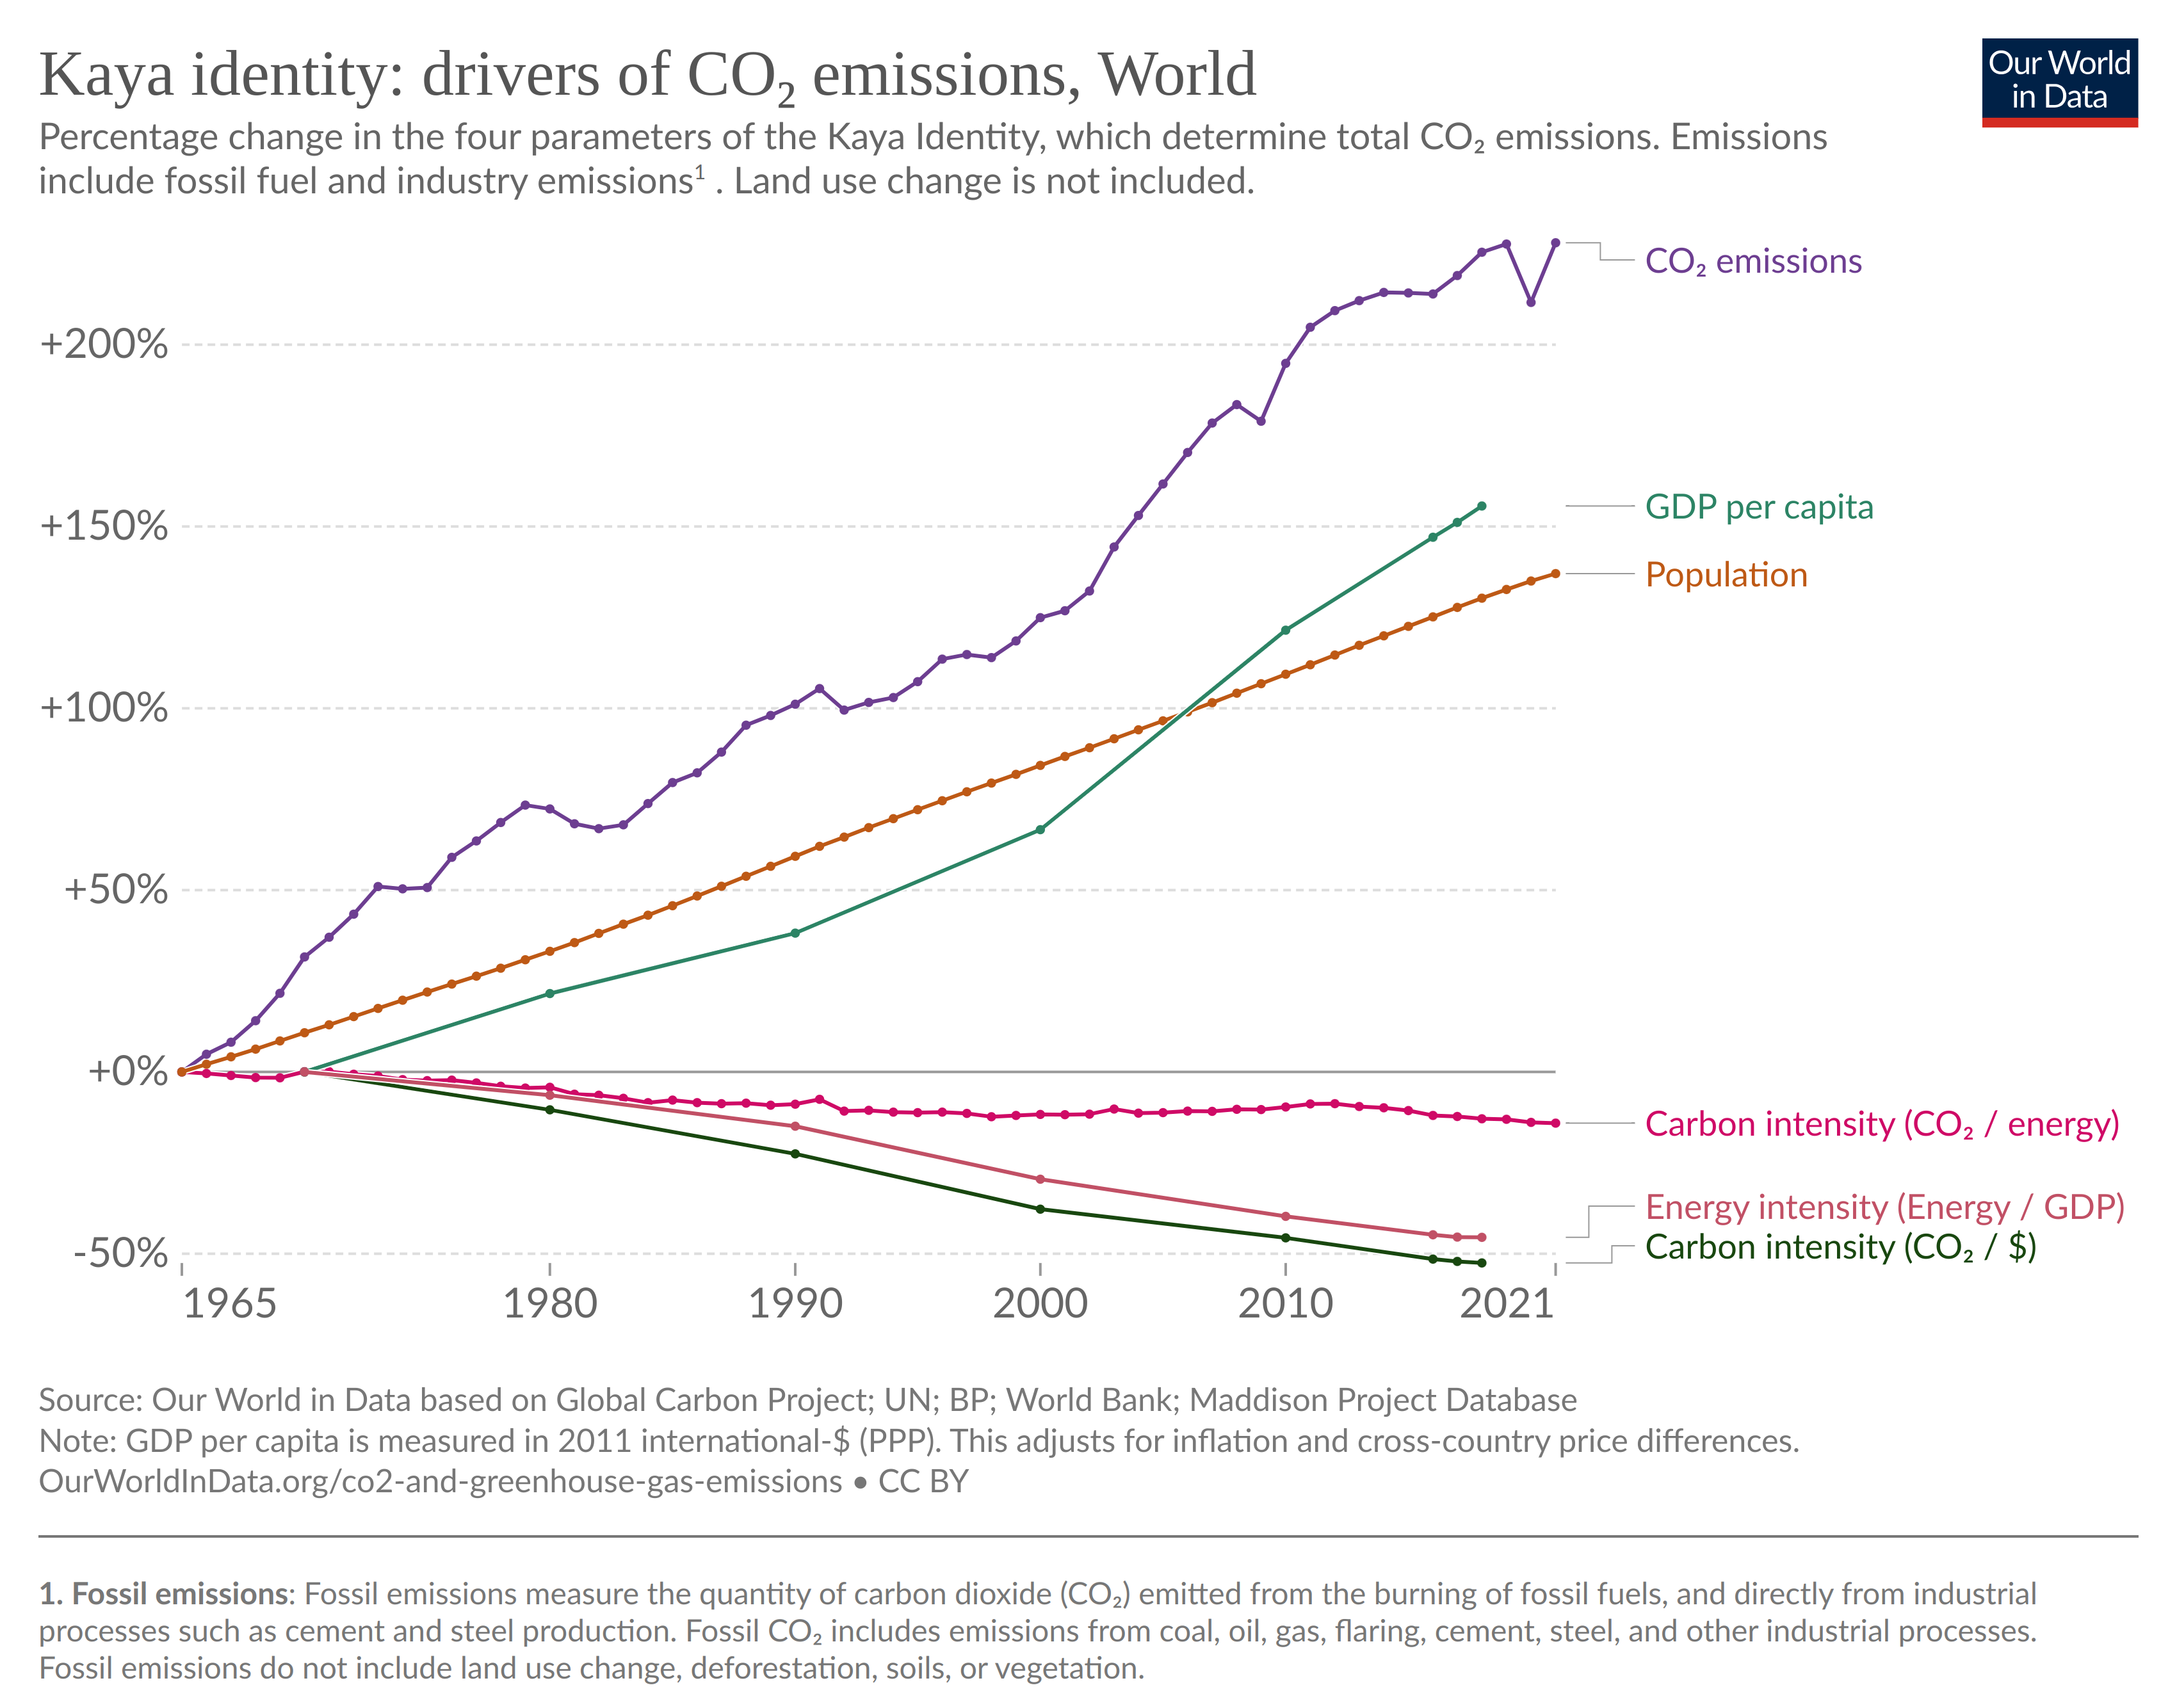
\includegraphics[width=0.55\textwidth]{figures/kaya-components.png}
    \caption{The Components of the Kaya Identity}
    \label{fig:kaya_components}
\end{figure}

\subsection{SSPs and RCPs}
\label{sec:ssps_rcps}

\textbf{Representative Concentration Pathways} (RCPs), are scenarios of future 
concentrations of greenhouse gases and other forcings. RCPs were used in the 
(\gls{IPCC}'s) Fifth Assessment Report.

The RCPs are named after their radiative forcing target level for the year 2100,
expressed in (W/m$^2$). There are four RCPs: 

\begin{itemize}
    \item \textbf{RCP 2.6}: This is a "peak and decline" scenario, where greenhouse gas
    emissions peak between 2010 and 2020, with substantial declines thereafter. By 
    2100, the additional radiative forcing is limited to 2.6 W/m$^2$.

    \item \textbf{RCP 4.5 and RCP 6}: These are stabilization scenarios where total radiative 
    forcing is stabilized before 2100 by applying a range of technologies and 
    strategies for reducing greenhouse gas emissions. The additional radiative 
    forcing in 2100 is 4.5 W/m$^2$ and 6 W/m$^2$, respectively.

    \item \textbf{RCP 8.5}: This is a rising radiative forcing pathway leading to 8.5 W/m$^2$ by 
    2100. This scenario assumes that emissions continue to rise throughout the 21st
    century.
\end{itemize}

These pathways provide inputs for climate model simulations to project future 
climate change. It's important to note that they're not predictions or forecasts,
but are plausible scenarios based on specific assumptions about future 
socio-economic development, technological changes, and policy interventions. 

The RPC approach has been extensively criticised by placing too much emphasis on
the most pessimistic of outcomes. As a result thereof, the \gls{IPCC} has
introduced a new set of scenarios for the Sixth Assessment Report, called the
\textbf{Shared Socioeconomic Pathways} (SSPs).\\


\noindent The SSPs link population growth and movement, technological development, energy
production and use, land use and cost to future greenhouse gas and aerosol
emissions into 5 different ``choices'' or scenarios that are as follows (directly
quoted):
\begin{itemize}
    \item \textbf{SSP1: Taking the Green Road}. World shifts towards a more sustainable
    path, common solutions to health and educational issues, economic growth
    places emphasis on human well-being. Greater equality results.
    \item \textbf{SSP2: Middle of the Road}. Social, economic and technological trends follow
    historical patterns leading to uneven growth. There is slow progress
    towards sustainable development goals.
    \item \textbf{SSP3: Regional Rivalry - A Rocky Road}. Nations put their own interests first
    at the expense of wider development and international action on sustainable
    development goals (e.g. health, education, climate).
    \item \textbf{SSP4: Inequality - A Road Divided}. Increasing inequality both across and
    within nations. Effectively the rich get richer and the poor get poorer.
    Conflict and unrest become increasingly common.
    \item \textbf{SSP5: Fossil-fuelled development - Taking the Highway}. Growth in innovation
    and competitive (but integrated) markets allows rapid technological progress.
    Strong investment in health and education. Development is fuelled by fossil
    fuel exploitation. Geo-engineering is a viable option (see section 
    \ref{sec:geoengineering})
\end{itemize}

The different SSPs lead to different emission levels (with SSP1 being the lowest
and SSP5 being the highest). Aerosol emissions are reduced in all SSPs.
It is important to note that none of these scenarios
are able to match the Paris Agreement goals without additional implementation of
mitigation strategies (carbon capture, geoengineering etc.).\\

For some lower-level details on the SSPs (GDP, GDP per capita, total energy 
demand, impact on the global mean surface temperature) see L12 slides 18 onwards or 
\href{https://www.sciencedirect.com/science/article/pii/S0959378016300681}{Riahi
\textit{et al.} 2017}.



\newpage
\section{Harnessing Wind Energy}
\label{sec:harnessing_wind}

As has become apparent in section \ref{sec:climate_policy}, there is a significant
need to reduce the carbon emissions from the energy sector. One of the ways to
achieve this is to substitute fossil fuels as an energy source for renewable
sources of energy. While sun and wind power are thought to be the ones most likely
to grow the fastest in the next decades, this section will focus on wind power
and how it can be harnessed. 

\subsection{Extracting Power from the Wind}
\label{sec:extracting_power_from_wind}

The main idea about wind power is that, by using a device (wind turbine) we are 
able to extract energy from the wind (kinetic energy) and transform it into some
other form of energy that is more useful to us (electrical power).\\

Let's consider a model in which air is an incompressible fluid (poor assumption),
with density $\rho$
the unperturbed wind is initially travelling with speed $V_1$ and swept cross-sectional
area $S_1$ and after passing through the wind turbine it is travelling with speed
$V_2$ and swept cross-sectional area $S_2$. See Figure \ref{fig:wind_turbine_model}.

\begin{figure}[ht]
    \centering
    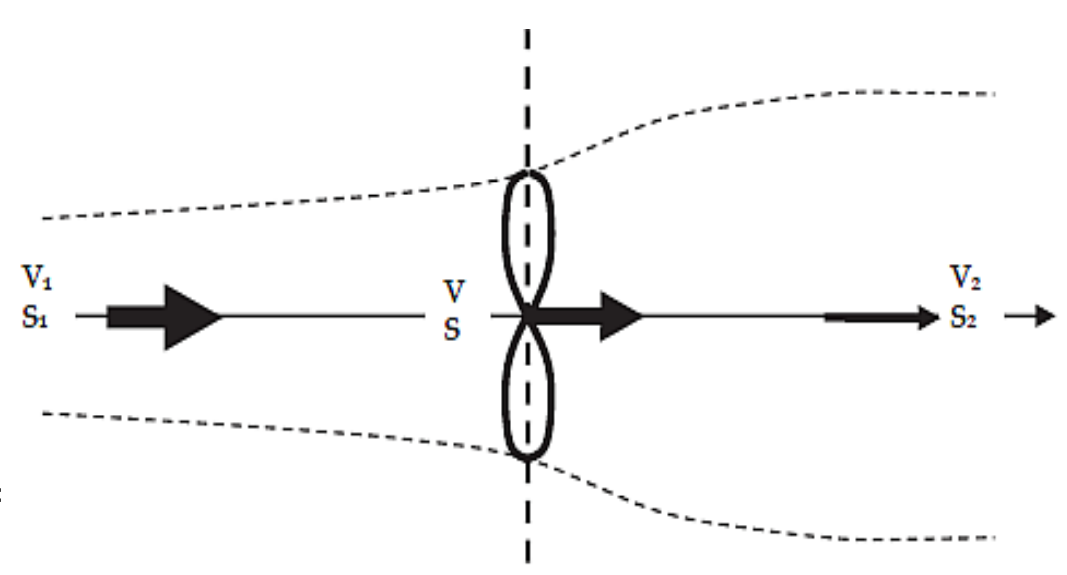
\includegraphics[width=0.65\textwidth]{figures/wind_turbine_model.png}
    \caption{Wind Turbine Model}
    \label{fig:wind_turbine_model}
\end{figure}

\noindent With this in mind we can note a few things. Firstly, the fact that the
turbine extracts kinetic energy suggests that $V_2 < V_1$. Secondly, as per conservation
of mass flow, we can write that
$$
\frac{dm}{dt} = \rho V_1 S_1 = \rho V_2 S_2 = \rho SV = \text{constant}
$$
and from it we can derive the power we are able to extract from the wind:
\begin{align*}
    \text{Force applied by wind} \quad & F = m \frac{dV}{dt} = \frac{dm}{dt} \Delta V
    = \rho SV (V_1 - V_2) \\
    \text{Power from wind} \quad & P = F \frac{dx}{dt} = \rho SV^2(V_1 - V_2)
\end{align*}

Similarly, we can write the power in terms of change of kinetic energy:
$$
P = \frac{1}{2} \frac{dm}{dt} (V_1^2 - V_2^2) = \frac{1}{2} \rho SV (V_1^2 - V_2^2)
$$
and equating the two expressions for power we get:
\begin{align*}
    \frac{1}{2} \rho SV (V_1^2 - V_2^2) &= \rho SV^2(V_1 - V_2) \\
    \frac{1}{2} (V_1 + V_2)\cancel{(V_1 - V_2)} &= V \cancel{(V_1 - V_2)}
\end{align*}
\begin{gather*}
    V = \frac{1}{2}(V_1 + V_2)\\
    \boxed{P = \frac{1}{4} \rho S(V_1^2 - V_2^2)(V_1 + V_2)}
\end{gather*}
so we have obtained a formula for the total available power to be extracted from
the wind.\\

It is evident however, that due to limtiations similar to those we encountered
in Carnot cycles in thermodynamics we will not be able to harness 100\% of all
available power. It therefore follows that we will be interested in how efficient
our wind turbine is, and therefore can define the \textbf{performance coefficient}
$C_p$. To do that we firstly introduce the concept of the kinetic power content, 
$W$ i.e. the power contained in a unit mass of air moving with initial speed $V_1$:
$$
W = \frac{1}{2}\frac{dm}{dt} V_1^2 = \frac{1}{2} \rho SV_1^3
$$
and so we define the performance coefficient as the power extracted from the wind
turbine divided by the kinetic power the wind had in the first place:
$$
C_p = \frac{P}{W} = \frac{\cancelto{\frac{1}{2}}{\frac{1}{4}\rho S}(V_1^2 - V_2^2)(V_1 + V_2)}
{\cancel{\frac{1}{2} \rho S}V_1^3} = \frac{(V_1^2 - V_2^2)(V_1 + V_2)}{2V_1^3}
$$
to which we can introduce the interference factor $b=V_2/V_1$ and make some 
substitutions:
\begin{align*}
    P &= \frac{1}{4} \rho S V_1^3 (1 - b^2)(1 + b) \\
    C_p &= \frac{1}{2}(1 - b^2)(1 + b)
\end{align*}
and finally we can plot the performance coefficient as a function of the interference
factor (see figure \ref{fig:performance_coefficient}).
\begin{figure}[h]   
    \centering
    \begin{tikzpicture}

        \begin{axis}[
            axis lines = left,
            xlabel = $b$,
            ylabel = {$C_p$},
            xmin=0, xmax=1,
            ymin=0, ymax=0.6,
            xtick={0,0.333, 0.5,1},
            ytick={0,0.2,0.4,0.6},
        ]
        \addplot [
            domain=0:1, 
            samples=100, 
            color=red,
        ]
        {0.5*(1-x^2)*(1+x)};
        % Vertical line at b=1/3 to show maximum point
        \addplot[black, thick, dotted] coordinates {(0.333, 0) (0.333, 0.593)};

        \end{axis}
    \end{tikzpicture}
    \caption{Performance coefficient as a function of interference factor}
    \label{fig:performance_coefficient}
\end{figure}

\noindent From the plot we can see that the maximum performance coefficient is
$C_p = 0.593$ and it occurs at $b=1/3$. This is the \textbf{Betz Limit} and it
is the maximum theoretical power fraction that can be extracted from a wind stream.
Analytically we can write:
$$
\frac{dC_p}{db} = \frac{1}{2} (1 - 3b)(1+b) \quad \implies \quad b = \frac{1}{3}
\quad \therefore V_2 = \frac{1}{3}V_1
$$
which using the above definition for $P$ we get:
$$
P = \frac{16}{27} \frac{\rho}{2} V_1^3 S
$$
and assuming a circular swept area of diameter $D$ i.e. $S = \pi D^2/4$ we get:
$$
P = \frac{16}{27} \frac{\rho}{2} V_1^3 \frac{\pi D^2}{4}
$$

\noindent In reality, just like with the Carnot cycle, it is not realistic to obtain this
maximum efficiency due to frictional losses in the rotor, drag due to blade surface
roughness and other mechanical imperfections. In practice, the maximum efficiency
is around 40-45\%.

\subsection{Wind-Speed Distributions}
\label{sec:windspeed_distributions}

In order to be able to estimate how much power will be able to be extracted from
the wind it is important to know the wind speed distribution as to place wind 
turbines in the most optimal of places.\\

We typically approximate the wind-speed distribution $f(V)$ as a Rayleigh distribution:
$$
f(V)_{\text{Rayleigh}} = \frac{V}{c^2} e^{-(V/c)^2} \quad \quad 0 \leq V < \infty
$$
and in some situations, the Weibull distrubution might be more appropriate:
$$
f(V)_{\text{Weibull}} = \frac{k}{c} \left(\frac{V}{c}\right)^{k-1} e^{-(V/c)^k}
\quad \quad 0 \leq V < \infty
$$
where $c$ and $k$ are distribution parameters. The Weibull goes to a Rayleigh
when $k=2$.\\

We can therefore use the Rayleigh distribution to estimate the average extractable
power. For a turbine operating in a flow of instantaneous speed $V$ the extractable 
power $P$ is:
$$
P = C_p \frac{V^2}{2} \frac{dm}{dt} = \frac{1}{2} C_p \rho S V^3
$$
and as per what we said before, we can find a mean for the power by using the mean
of the distribution of wind speeds:
\begin{align*}
    \overline{P(V)} &= C_p \int_{V_{\text{min}}}^{V_{\text{max}}} P(V) f(V)_{\text{Rayleigh}} dV\\
    &= C_p \int_0^\infty \frac{\rho S V^3}{2} f(V)_{\text{Rayleigh}} dV\\
    &= \frac{C_p \rho S}{2} \int_0^\infty V^3 f(V)_{\text{Rayleigh}} dV\\
    \Aboxed{\overline{P(V)} &= \frac{C_p \rho S}{2} \overline{V^3}}
\end{align*}

Note that $\overline{V^3}$ is not the same as $\overline{V}^3$. In this case, we
use $\overline{V^3} = c^3 3\sqrt{\pi}/4$ for the equations above.\\

It therefore follows that at the Beltz Limit:
$$
\boxed{
\overline{P(V)}_{\text{max}} = \frac{16}{27} \frac{\rho}{2} \frac{\pi D^2}{4}
\frac{6}{\pi} \overline{V}^3 = \rho \left( \frac{2}{3} D \right)^2 \overline{V^3}}
$$

Another factor to bear in mind is the fact that the wind speed is not constant
on the vertical axis: it increases with height. This is in fact the reason why
wind turbines have been getting taller and larger in diameter over the years.

A good model for the vertical distribution of speeds is a logarithmic profile 
as follows:
$$
\boxed{V(z) = k \ln \left(\frac{z}{z_0}\right)}
$$
where $k$ is a constant and $z_0$ is the \textbf{roughness length} - a measure
of the height above the surface at which the windspeed theoretically becomes zero.
Roughness length is indeed determined by the roughness of ther surface, i.e. how
much of an impediment does it pose to the wind travelling above it.

\begin{table}[h]
    \centering
    \begin{tabular}{c|c}
        \textbf{Surface} & \textbf{Roughness Length (m)}\\
        \hline
        Sand & 0.0001-0.001\\
        Open Sea & 0.005\\
        Grass & 0.01-0.1\\
        Suburban & 0.2-0.4\\
        Urban & 0.35-0.8\\
        Forest & 0.9-1\\
    \end{tabular}
    \caption{Roughness Lengths}
    \label{tab:roughness_lengths}
\end{table}

\subsection{Issues with Wind Power}
\label{sec:issues_with_wind_power}

There are a number of issues with wind power that have to be considered. Here is
a non-exhaustive list:
\begin{itemize}
    \item Wind supply is not constant, meaning that there will be times when generation
    is needed but is not able to be provided, and times of excess generation. This
    has to be addressed by having a backup power source, or by having a way to store
    the excess energy.
    \item They are noisy and can be an eyesore. 
    \item Power transmission/distribution is an issue. Wind farms are typically
    located in remote areas, meaning that the power has to be transmitted over long
    distances, leading to potential losses.
    \item There is a non-zero carbon impact of buliding and replacement of wind
    turbines. An average lifespan for a wind turbine is 10-20 years.
    \item Large scale deployment of wind turbines create wake effects, i.e. the
    performance of a turbine is affected when it is behind another one. Turbine 
    separation must be 5-10x rotor diameter.
\end{itemize}

% Section glossary




\newpage
\section{Solar Energy}
\label{sec:SolarEnergy}

In previous sections we have seen the importance of an increase in renewable 
energy generation in order to reach climate goals. In the previous section we 
concentrated on wind power, in this one we will look at solar power. \\

Near the beginning of the course we noted that \gls{TSI} at \gls{TOA} is 
$\sim$ 1360 W/m$^2$, which if averaged over the whole Earth is $\sim$ 240 W/m$^2$
when accounting for \hyperlink{glo:albedo}{albedo}, and \textbf{in total 120 PW}
(global electricity consumption is $\sim$ 3 TW, i.e. much smaller). For these
figures, we assumed that there is no atmospheric absorption or scattering in
\gls{SW}. Remember of course that this is not quite the case - \gls{SW} is mostly
unaffected by the atmosphere but not fully. See fig \ref{fig:transmitted_radiation} \\

Let's examine this assumption a bit more closely. As per section \ref{sec:opticaldepth},
we had a definition of optical depth, in that case just for an absorbing atmosphere.

It is apparent as per fig \ref{fig:transmitted_radiation} that the atmosphere is
not just absorbing but also scattering, especially in the \gls{SW}. As a result we
will modify the definition for optical depth to replace the mass absorption 
coefficient for the \textbf{mass extinction coefficient} $\kappa_{\text{e}\lambda}$:
$$
\boxed{
    \tau_\lambda = \int_0^z \kappa_{\text{e}\lambda}(z) \rho_\text{a}(z) dz
}
\quad \text{where} \quad \kappa_{\text{e}\lambda} = \kappa_{\text{a}\lambda} + 
\kappa_{\text{s}\lambda}
$$
so the solar radiation reaching the surface becomes:
$$
I_{\text{surface}} = I_{\text{TOA}} e^{-\tau_\lambda} 
$$
so it becomes aparent that \textbf{path length} and therefore how much atmosphere
is interacting with the sunlight before reaching the surface is important in 
determining how much of it will be available at the surface. 

\noindent Before moving on, we must first define some concepts that will allow
us to progress. \\


\subsection{Some Definitions}
\label{sec:solar_definitions}

\noindent To account for path length, for solar energy applications we will often
encounter the concept of \textbf{air mass} (AM). The concept of air mass is a way to
quantify the amount of atmospheric matter (such as air molecules, aerosols, etc.)
that sunlight must traverse before it reaches the Earth's surface.
This path length of sunlight through the atmosphere is directly related to the 
amount of scattering and absorption the sunlight undergoes, which impacts its 
intensity by the time it reaches the surface.

The AM is defined as the ratio of the actual path length that sunlight travels 
through the Earth's atmosphere relative to the path length it would travel if 
the sun were directly overhead, i.e. at zenith. At zenith, sunlight travels the
shortest possible path through the atmosphere, and so this path length serves 
as our baseline (AM=1) for defining air mass. We define AM mathematically as:

$$
\boxed{
    \text{AM} = \sec (\theta_z) \quad \implies \quad I_{\text{surface}} =
    I_{\text{TOA}} e^{-\tau_\lambda \sec (\theta_z)}
}
$$
note that an air mass of 0 implies extra-terrestrial, \gls{TOA} solar irradiance
at the surface, i.e. no atmosphere.

\noindent A useful number for air mass is 1.5, which is the average air mass
at a latitude in a "temperate climate" $\sim$ 42$^\circ$ latitude (e.g. Barcelona).
This is useful since population tends to be closer to latitudes like these rather 
than the equatior or poles.\\

\noindent In the above equation we used $\theta_z$ to denote the \textbf{solar
zenith angle}, this is the angle between the direction of
the sun and the vertical (zenith direction). When the sun is directly overhead,
$\theta_z = 0$ and the air mass is 1. As the sun moves away from zenith, $\theta_z$
increases, and the sunlight has to traverse a longer path through the atmosphere,
thus increasing the air mass.\\

\noindent Total solar radiation at the surface can be broken down into two 
components: \textbf{direct} and \textbf{diffuse} radiation. 

\textbf{Direct Radiation}: This is the portion of solar radiation that comes 
straight from the direction of the Sun without undergoing any kind of scattering
or reflection. It follows a direct path from the Sun to the Earth's surface. 
This is of special interest to technologies like concentrating photovoltaics 
(CPV), which work best with direct sunlight (they use concentrating optics so
they track the sun).

\textbf{Diffuse Radiation}: This is the portion of solar radiation that has been
scattered in various directions by molecules, aerosols, and clouds in the 
Earth's atmosphere. Instead of coming from a single direction, like the Sun, 
diffuse radiation comes from multiple directions. This scattered light reaches
the Earth's surface from different angles and is important for standard 
photovoltaic (\gls{PV}) panels which can absorb sunlight from various directions (these
tend to be fixed so don't track the sun). \\

\noindent The following two terms are not crucial to know, but can be useful for a better 
understanding of the topic and its literature.

The term \textbf{global radiation} can sometimes cause confusion, as it might suggest 
something related to the entire globe. However, "global" radiation
simply refers to the total amount of solar radiation reaching a specific location
on Earth's surface, i.e., it's the sum of direct and diffuse radiation at said point.

Another term that might appear is \textbf{Direct Normal Irradiance} (DNI). 
This refers to the amount of solar radiation received per unit area by a surface 
that is always held perpendicular (or normal) to the rays that come in a straight 
line from the direction of the sun. This is particularly relevant for solar 
concentrator systems, which aim to maximize their exposure to direct radiation.

\subsection{Photovoltaic Fundamentals}
\label{sec:PV_fundamentals}

\noindent A number of further concepts are introduced in Lecture 14b, most of which
are not crucial to know for the exam. Here follows a brief summary of the most
important ones.\\

\textbf{Solar Materials}: Different materials have different uses when it comes to 
harnessing solar energy. For solar \textbf{thermal} applications, metals or black solids 
are often used because they are excellent at absorbing sunlight and converting 
it into heat. For solar chemical applications, plants are used in processes like 
photosynthesis, where sunlight is used to convert carbon dioxide and water into 
glucose and oxygen. Sometimes other chemicals are used for solar chemical
processes as well, such as in the production of hydrogen from water using
photoelectrochemical (PEC) cells. \\

\textbf{Photovoltaics}: Photovoltaic (\gls{PV}) materials are used in solar panels to convert 
sunlight directly into electricity. The key material in PV cells is a semiconductor, 
often silicon, which is 'doped' with impurities to create a so-called p-n junction 
with properties favorable for solar energy conversion. The band-gap of this 
semiconductor material is crucial - it must be suitable to absorb the energy from 
incoming solar photons, which can then excite electrons across the band-gap, 
creating an electric charge.\\

\noindent The band gap is the energy difference between the valence band (where electrons 
are normally located) and the conduction band (a higher energy level where 
electrons can move freely). When a photon with energy equal to or greater than 
the band gap hits the PV cell, it can excite an electron from the valence band 
to the conduction band, creating an electron-hole pair. The `size' of the band gap
greatly affects the performance of the PV cell. A large band gap will be excited by
high energy photons and will produce a high voltage, as they leave behind a hole
in the valence band and there is a large difference between the two (potential 
difference). However, a large band gap will not be excited by as many electrons
(the lower energy ones, higher wavelength) so the current of such cell will be lower.\\

\textbf{Photogenerated Charges}: Once the solar photons have been absorbed and the 
electrons are excited across the band-gap, these photogenerated charges 
(electron-hole pairs) need to be separated to prevent them from simply recombining. 
The p-n junction and an associated electric field help in this charge separation. 
Asymmetric contacts made to an external circuit then allow these charges to flow 
as an electric current.\\

\textbf{Power and Efficiency}: The power produced by a PV cell is the product of the 
photovoltage (the voltage generated by the photovoltaic effect) and the 
photocurrent (the current generated by the separated charges). The maximum power 
point of a cell is where the product of the photovoltage and photocurrent is 
greatest. The power conversion efficiency of a PV cell, meanwhile, is the ratio 
of the power (or power per unit area) that is converted into useful work 
(electricity), divided by the incident power (or irradiance) from the sun. 
Consistency in units is crucial when calculating efficiency.\\

% A graph showing voltage, current and power curves for a PV cell. Y axis is AU,
% X axis i band gap energy. The curves are labelled 
\begin{figure}[h]
    \centering
    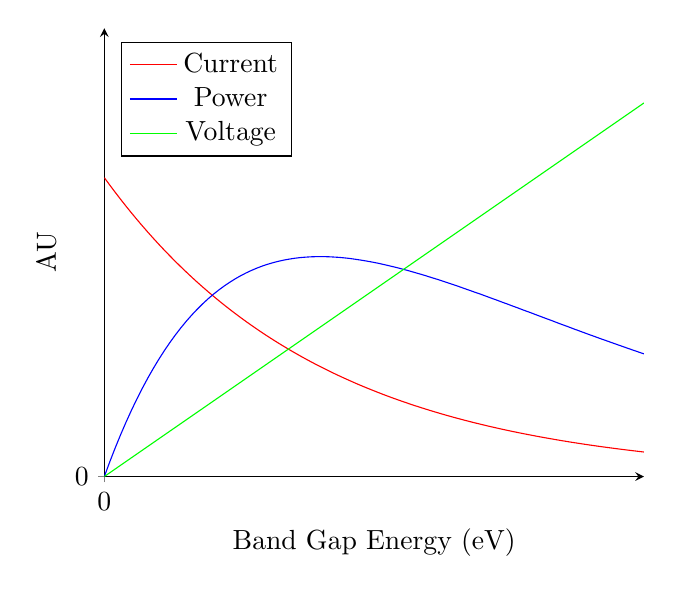
\begin{tikzpicture}
        \begin{axis}[
            axis lines = left,
            xlabel = {Band Gap Energy (eV)},
            ylabel = {AU},
            xmin = 0, xmax = 2.5,
            ymin = 0, ymax = 1.5,
            xtick={0},
            ytick={0},
            legend pos = north west,
        ]
        %Current curve
        \addplot [
            domain=0:2.5, 
            samples=100, 
            color=red,
        ]
        {exp(-x)};
        \addlegendentry{Current}
        %Power curve
        \addplot [
            domain=0:2.5, 
            samples=100, 
            color=blue,
            ]
            {2*x * exp(-x)};
        \addlegendentry{Power}
        %Voltage curve
        \addplot [
            domain=0:2.5, 
            samples=100, 
            color=green,
            ]
            {0.5*x};
        \addlegendentry{Voltage}
        \end{axis}
    \end{tikzpicture}
    \caption{Current, voltage and power curves for different band gaps. Note
    that these are estimates and not to scale.}
    \label{fig:SQ_curves}
\end{figure}


\subsection{PV Technology}
\label{sec:PV_technology}

In the lecture a number of PV technologies, each with their advantages/drawbacks
were introduced. Here follows a summary of the most important ones.\\

\textbf{Single-Junction Silicon Cells}: These are the most commonly used type of 
PV cell and are typically composed of monocrystalline or polycrystalline silicon. 
They rely on a single semiconductor material (silicon) with a specific band gap. 
This restricts the range of light wavelengths that can be absorbed and turned 
into electrical energy, hence limiting the maximum theoretical efficiency to 
about 33.7\% under standard test conditions\footnote{Said standard test conditions
try to replicate what the cell would experience under 1.5 SM, i.e. 1000 W/m$^2$
and a particular frequency spectrum. This spectrum can be found online but all that
is worth knowing is that it tries to replicate real-world conditions and that it
is normalised for 1000 W/m$^2$.} (known as the Shockley-Queisser 
limit). In practice, the efficiencies achieved are usually around 15-20\%, with 
the highest efficiencies nearing 26\%.

\textbf{Multi-Junction Cells}: These PV cells are composed of multiple layers, 
each made from different semiconductor materials with different band gaps. This 
allows the cell to absorb a broader range of light wavelengths, enhancing its 
efficiency. Each layer in the multi-junction cell is designed to absorb a 
specific range of the solar spectrum, allowing it to capture more of the 
incoming solar energy than a single-junction cell could. As a result, 
multi-junction cells can achieve efficiencies approaching 50\%. However, they 
are also more complex and expensive to manufacture.

\textbf{Alternative Material-Based Cells}: These are a diverse group of emerging 
PV technologies that use materials other than traditional semiconductors. This 
includes organic (plastic) solar cells, dye-sensitized solar cells, and 
perovskite solar cells. These technologies offer the potential for lower costs 
and more flexible applications, but they currently face challenges related to 
efficiency, stability, and scaling.


\newpage
\section{Geoengineering Our Climate}
\label{sec:geoengineering}

For this course we will take the following definition of geoengineering:
\begin{tcolorbox}
    \centering
    \textit{``The deliberate, large-scale intervention in the 
    Earth's natural systems to counteract climate change.''}
\end{tcolorbox}

Two main types of geoengineering are considered:
\begin{itemize}
    \item \textbf{Carbon Dioxide Removal (CDR)}: The removal of \ce{CO2} from 
    the atmosphere in an attempt to minimise the atmosphere's overall greenhouse
    effect and hence reduce global mean surface temperature. This increases the
    OLR side of the energy-balance equation. Examples include afforestation,
    ocean fertilisation and direct air capture.
    \item \textbf{Solar Radiation Management (SRM)}: The reflection of incoming
    solar radiation away from the Earth in an attempt to reduce the amount of
    energy absorbed by the Earth's surface. This reduces the absorbed solar
    radiation side of the energy-balance equation. Examples include stratospheric
    aerosol injection, low cloud albedo enhancement and space-based reflectors.
\end{itemize}

Before we discuss the various methods of geoengineering, we must introduce a 
concept that we will have to bear in mind throughout the rest of this section - 
\textbf{EATS}. This stands for the following:

\begin{itemize}
    \item \textbf{E}ffectiveness: Is the proposed method going to have a significant,
    measurable impact on the climate system?
    \item \textbf{A}ffordability: Is the proposed method likely to be affordable?
    \item \textbf{T}imeliness: Is the proposed method likely to be available in
    time to prevent dangerous climate change? How mature is this technology?
    \item \textbf{S}afety: Is the proposed method likely to have any negative
    side-effects?
\end{itemize}
And lastly (not in this mnemonic) we should also consider legality, and feasibility,
international cooperation, public perception etc.

\subsection{Carbon Dioxide Removal}
\label{sec:CDR}

In this section we will discuss various examples of \gls{CDR}. \\

\noindent \textbf{Bio-Energy with carbon capture and storage (BECCS)}: This is a combination
of two technologies - bio-energy and \gls{CCS}. The idea is to grow biomass (trees), burn
it to generate energy and then capture the \ce{CO2} emitted during combustion through 
\gls{CCS} techniques. The captured \ce{CO2} is then transported and stored underground
or under the sea. This process therefore acts as a net \textbf{carbon sink} - it removes
\ce{CO2} from the atmosphere and stores it underground. This is sometimes referred 
to as ``negative emissions''. 

However, it is worth noting that implementing this is not without its challenges.
Mainly, this requires a vast amount of land to grow the biomass on, which 
negatively impacts food security and biodiversity. Furthermore, the time-scale
is not particularly favourable and there are significant monetary costs involved.\\

\noindent \textbf{Enhanced Rock Weathering}: This is a climate change mitigation 
strategy that accelerates the natural process of weathering to remove carbon 
dioxide from the atmosphere. It involves pulverizing rocks rich in silicate 
minerals, like basalt or olivine, and spreading them over large areas. The 
increased surface area of the powdered rock allows for faster chemical reactions 
with \ce{CO2}, locking it away in stable forms such as bicarbonate ions. This not 
only reduces atmospheric \ce{CO2} levels but also replenishes soil nutrients for 
crops and promotes plant growth, which further absorbs \ce{CO2} (feedback). Furthermore,
when eventually these are washed away by rivers into the ocean these are the ``right
kind'' of carbonates that help reduce ocean acidification.
Despite its potential, the method poses challenges, including the energy-intensive 
process of mining and grinding rocks and the potential reduction of albedo due 
to the dark rocks.\\

\subsection{Solar Radiation Management}
\label{sec:SRM}

\noindent \textbf{Marine Cloud Brightening}: This is a proposed form of \gls{SRM} 
that levereges the Twomey effect (see Section \ref{sec:aerosol-radiative-forcing}),
i.e. the indirect effect. The idea is to spray aerosols into the atmosphere which,
in areas of marine stratocumulus (this occurs especially to the west of continents)
will increase the number of cloud droplets and hence increase the cloud albedo 
significantly. This is suggested to be done by having a fleat of ships that pump
sea salt into the atmosphere. This will increase the amount of solar radiation 
reflected back
into space, reduce the amount of solar radiation absorbed by the Earth's surface
and therefore reduce global mean surface temperature. \\

However, this method is not without its challenges. It is not clear whether
this system is really scalable. Secondly, there might be hidden carbon costs 
(having a fleat of ships pumping sea salt into the atmosphere is not exactly
carbon neutral). 


\newpage
\glsaddall
\printglossaries

\bibliographystyle{plain}
\bibliography{references}
\end{document}
